\documentclass[12pt]{report}

% ====== 1. Basic Configuration ======
\usepackage[T1]{fontenc}
\usepackage[utf8]{inputenc}
\usepackage{natbib}
\usepackage[french,english]{babel}
\usepackage{pifont}
\newcommand{\cmark}{\ding{51}} % checkmark
\newcommand{\xmark}{\ding{55}} % cross

% ====== 2. Math and Science Packages ======
\usepackage{amsmath, amsfonts}
\usepackage{algorithm}%
\usepackage{algorithmicx}%
\usepackage{algpseudocode}%

% ====== 3. Graphics and Tables ======
\usepackage{graphicx}
\usepackage[pdftex]{hyperref}
\usepackage{caption, subcaption}
\usepackage{float}
\usepackage{booktabs}
\usepackage{array, tabularx}
\usepackage{longtable, multirow}




% ====== 5. PGF/TikZ Configuration ======
\usepackage{pgfplots}
\pgfplotsset{compat=1.18} % SOLVES YOUR WARNING
\usepackage{tikz}
\usetikzlibrary{arrows, shapes, positioning}
\tikzstyle{block}=[draw opacity=0.7, line width=1.4cm]

% ====== 6. Page Layout ======
\usepackage[top=2cm, bottom=2cm, left=3cm, right=2cm]{geometry}
\usepackage{fancyhdr}
\usepackage{afterpage}

% ====== 7. Other Packages ======
\usepackage{textcomp}
\usepackage{pdflscape}
\usepackage{pdfpages}
\usepackage[nottoc]{tocbibind}
\usepackage{calligra, frcursive, xcolor}
\usepackage{pifont}
\usepackage[most]{tcolorbox}
\usepackage{fancyvrb}
\usepackage{listings}
\usepackage{soul}


% ====== 8. Hyperref Setup ======
\hypersetup{
	colorlinks,
	linkcolor=blue,
	citecolor=blue,
	urlcolor=blue
}

% ====== 9. Document Settings ======
\linespread{1.3}
\renewcommand{\footrulewidth}{0.3pt}
\DeclareUnicodeCharacter{200B}{}

% ====== 10. Custom Commands ======
\providecommand*{\figurename}{}
\renewcommand*{\figurename}{Figure}
\providecommand*{\tablename}{}
\renewcommand*{\tablename}{Table}

\begin{document}

	\providecommand*{\figurename}{}
	\renewcommand*{\figurename}{Figure}
	\providecommand*{\tablename}{}
	\renewcommand*{\tablename}{Table}
	%%%%%%%%%%%%%%%%%%%%%%%%%%% Cover page %%%%%%%%%%%%%%%%%%%%%%%%%%%%%%%%%
	\thispagestyle{empty}
\begin{center}
	\begin{title}
		\textbf{\uppercase{ People's Democratic Republic of Algeria }} \\[0.2cm]
		\textbf{\uppercase{ MINISTRY OF HIGHER EDUCATION AND SCIENTIFIC RESEARCH }} \\[0.5cm]
		\textbf{\uppercase{ UNIVERSITY MUSTAPHA STAMBOULI OF MASCARA}}
	\end{title}
	\begin{figure}[H]
		\centering
		\label{logo_UD}
\includegraphics[width=0.2\textwidth]{Figures/Logo_UM.jpg}
	\end{figure}
	{\large Faculty of Exact Sciences} \\[0.2cm]
	{\large Department of Computer Science} \\[0.2cm]
	{\large Dissertation } \\[0.2cm]
	{\ Submitted in partial fulfilment of the requirements for Master degree in Computer Science} \\[0.2cm]
	{\large Option: Intelligent Systems Engineering }\\[0.5cm]
	
    {\large Entitled} \\[0.3cm]
%\hline	
%    \\[0.7cm]
	{\LARGE {\textbf{Enhancing Reasoning Capabilities of Retrieval-Augmented Generation (RAG) in LLM-Based Agents for Legal and Juridical Data.}}}
	\\[0.7cm]
%\hline
%	 \\[0.5cm]

	{\large Presented by \textbf{Boudjenane Zoubida Asmaa} }\\[0.5cm]

\end{center}
Jury:\\
\begin{tabular}{llll}
	President    &  SMAIL Omar & Professor & University of Mascara\\
	Director     &  Mohammed SALEM & Professor & University of Mascara\\
	Examiner     & 	MAHMOUDI Laouni & Professor	& University of Mascara\\
	Examiner	 &  BOUFERA Fatma & Professor  & University of Mascara\\

\end{tabular}
\vfill
\begin{center}
	
	\it{2024/2025}
\end{center} % Cover page
	%\includepdf{Page_de_garde.pdf} % Cover page from pdf file 
	%%%%%%%%%%%%%%%%%%%%%%%%%%%% Acknowledgements %%%%%%%%%%%%%%%%%%%%%%%%%%
	\chapter*{Acknowledgements}
\thispagestyle{empty}
%\addcontentsline{toc}{chapter}{Acknowledgments}
%%%%%%%%%%%%%%%%%%%%%%%%%%%%%%%%%%%%%%%%%%%%%%%%%%%%%%%%%%%
\begin{center}
	
	
	First of all, praise and thanks to Allah Almighty for giving us all the patience, courage, will and motivation that allowed us to accomplish this work.\\ 
	\vspace{0.3cm}
	
	My deepest gratitude goes to my supervisor, \textbf{Mr Salem Mohamed } for his patient guidance, insightful feedback, and continuous encouragement throughout the course of this work .\\
	\vspace{0.3cm}
	 I would like to express my sincere gratitude to the members of the jury for their valuable time and insightful feedback:
	 
	 \begin{itemize}
	 	\item \textbf{Prof. SMAIL Omar },  at University of Mascara.
	 	\item \textbf{Prof. MAHMOUDI Laouni}, at University of Mascara.
	 	\item \textbf{Prof. BOUFERA Fatma}, at University of Mascara.
	 	
	 \end{itemize}
	 
	 Their rigorous examination and constructive suggestions have significantly improved this work.\\
	\vspace{0.3cm}
    I am also especially thankful to my parents, family, and friends for their unwavering support, love, and motivation at every step of this journey. \\
    \vspace{0.3cm}
    I would like to thank everyone who helps me to improve my work. and who gave me any remark that helped me to perfect this manuscript.\\
	\vspace{0.3cm}
	All the teachers of the University MUSTAPHA STAMBOULI DE LA WILAYA MASCARA For the good contribution of this work.
\end{center}

% Acknowledgements page
	%%%%%%%%%%%%%%%%%%%%%%%%%%%% Dedication %%%%%%%%%%%%%%%%%%%%%%%%%%%%%%%%%
	\newpage
	\thispagestyle{empty}
\begin{tikzpicture}[remember picture, overlay]
	\node at (current page){
		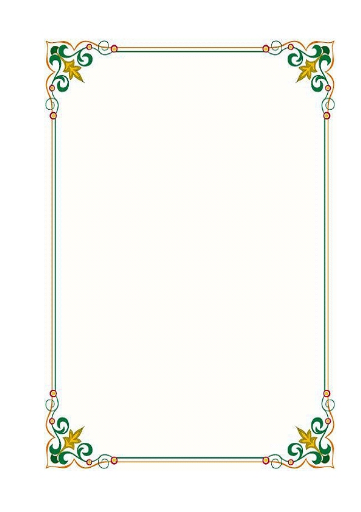
\includegraphics[width=\paperwidth,height=\paperheight]{Figures/bgg4.png}} ;
\end{tikzpicture}
\vskip15mm
\begin{center}
	\resizebox{6cm}{1.1cm}{\calligra Dedication} 
\end{center}
\vfill 
\begin{center}
	\parbox{.85\linewidth}{\centering 
		\baselineskip=8mm 
		\fontfamily{pzc}\selectfont 
		\Large 
This work is dedicated with deep love and gratitude to:
\\[5mm]
My dear parents,
whose unwavering support, sacrifices, and constant prayers have been the foundation of everything I’ve achieved. Your belief in me gave me the strength to persevere through every challenge.
\\[5mm]
My supervisor, Mr. Salem Mohamed,
whose patient guidance, insightful feedback, and continuous encouragement made this journey not only possible but meaningful. Your dedication, expertise, and belief in my potential have left a lasting impact on me both academically and personally.
\\[5mm]
My beloved sister Boudjenane Fatima Zahra,
for being my greatest cheerleader and my constant source of emotional support. Your encouragement and care during the toughest moments meant the world to me.
\\[5mm]
My wonderful friend nial hadjer,
for always being there with kind words, late-night conversations, and unshakable support.
\\[19mm]
}
\end{center}
\vfill 
\thispagestyle{empty}% Dedication page
	%%%%%%%%%%%%%%%%%%%%%%%%%%%% Abstracts in Arabic, English and French %%%%%
	%The abstract pdf file is obtained by compiling separately the abstract.tex file, due to the conflict between the Arabic language in the abstract and the hyperref package
	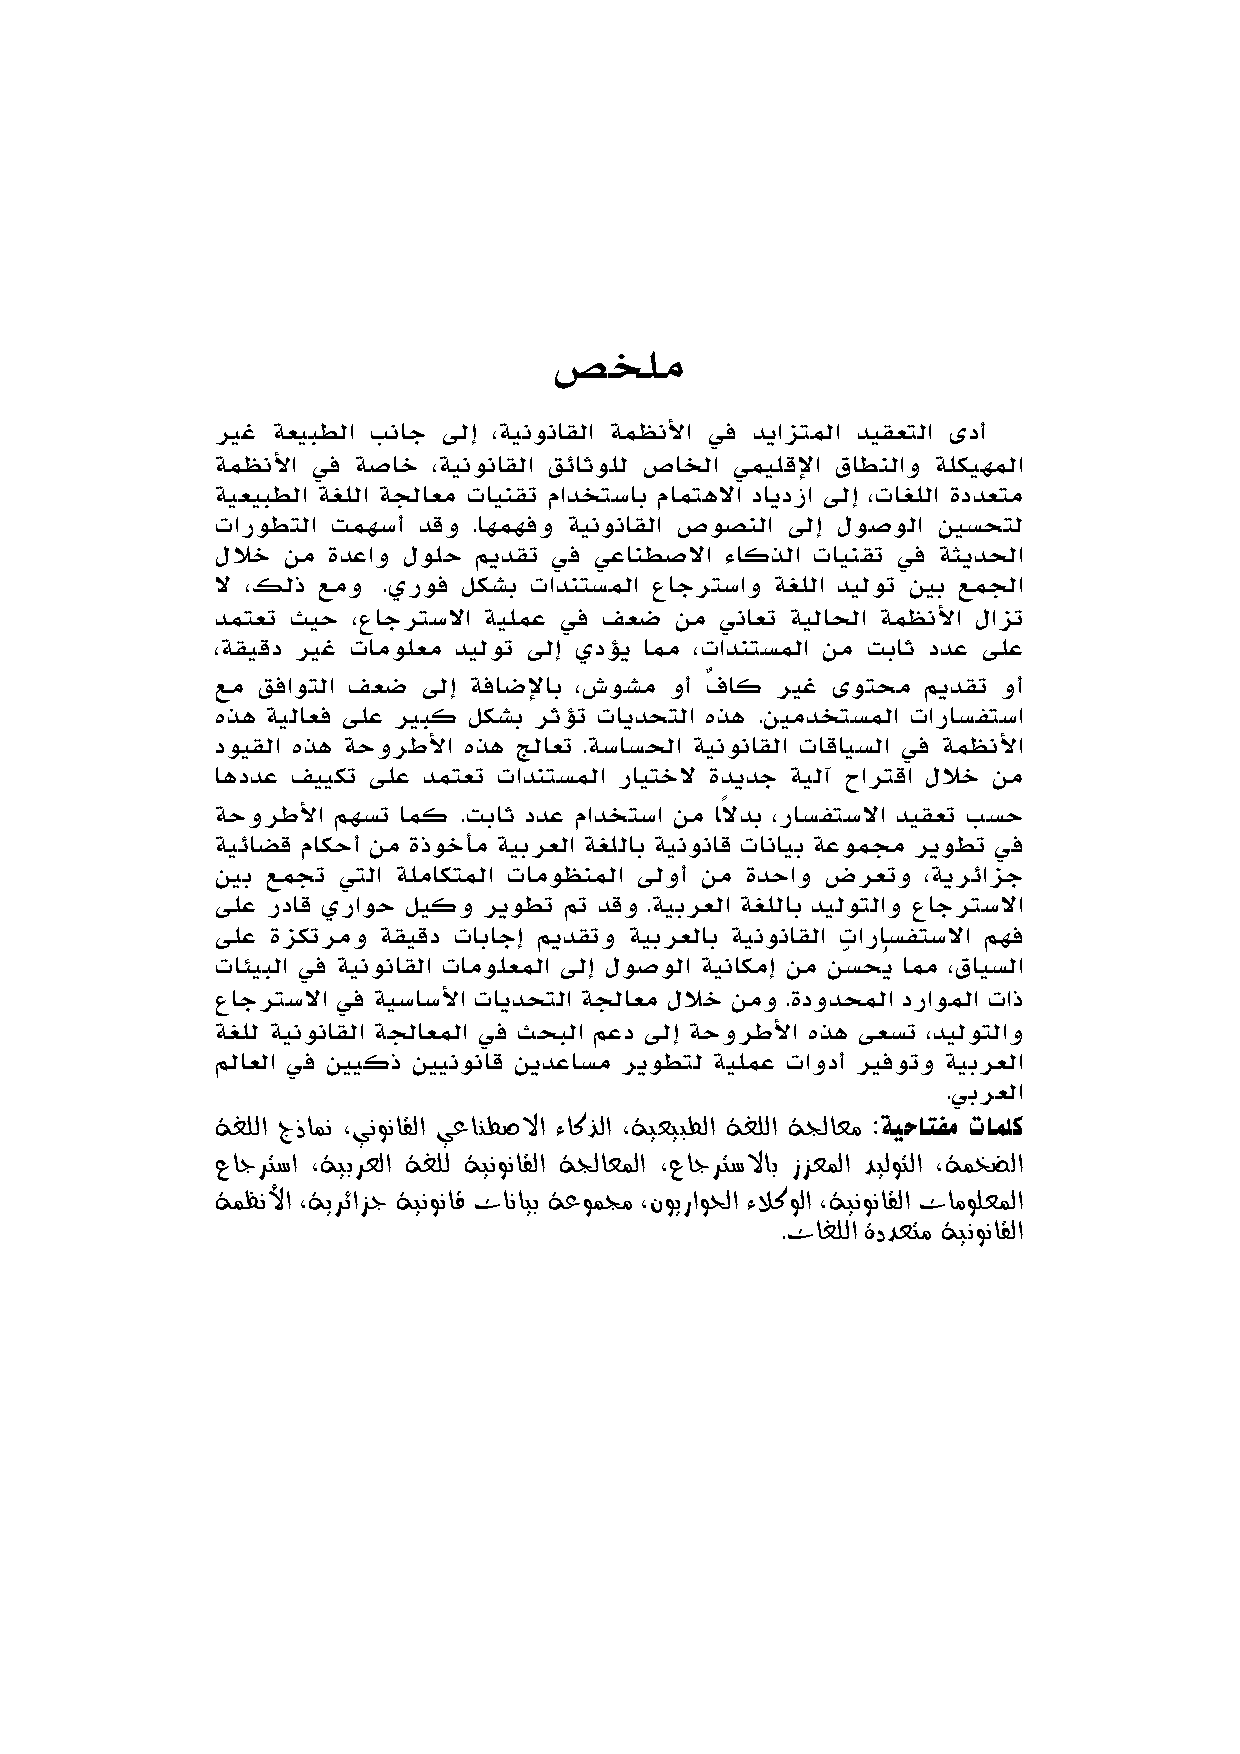
\includepdf[pages=-]{Abstract.pdf}
	%%%%%%%%%%%%%%%%%%%%%%%%%%%% Copyright declaration %%%%%%%%%%%%%%%%%%%%%%%
	% Images sources for copyright purposes 
	%\begin{landscape}
	\thispagestyle{empty}
	\begin{center}
		\Huge{\textbf{Sources of Images}} \\
		\normalsize{\textit{for Copyright purposes}}
	\end{center}
	Figure 1.1 from \url{https://blog.dataiku.com/nlp-metamorphosis} \\
	Figure 1.2 from \url{www.dmice.ohsu.edu/hersh/ohsu-pathology-20.pdf} \\
	Figure 1.3 from \url{https://w.wiki/3sAW} \\
	Figure 1.4 from \url{www.researchgate.net/publication/336092695_Densely_Connected_Convolutional_Networks_With_Attention_LSTM} \\
   Figure 1.5 from \href{https://www.medium.com/huggingface/encoder-decoders-in-transformers-a-hybrid-pre-trained-architecture-for-seq2seqaf4d7bf14bb8}{Medium article  transformers}\\
	Figure 1.6 from \href{https://medium.com/@anishnama20/exploring-the-power-of-encoder-decoder-models-pros-cons-and-applications-8bfbe2e66e76}{Medium article on encoder-decoders }	\\
	Figure 1.7 from \url{arxiv.org/abs/2307.09288} \\
	Figure 2.1 from \url{https://arxiv.org/abs/2312.10997} \\
	Figure 2.2 from \href{https://www.researchgate.net/figure/High-level-overview-of-a-possible-solution-using-RAG-and-a-multi-modal-in-context_fig1_380540048}{RAG } \\
   Figure 3.1 from \url{https://ai.gopubby.com/advanced-rag-techniques-unlocking-the-next-level-040c205b95bc} \\
	Figure 3.2 from \url{www.evidentlyai.com/ranking-metrics/precision-recall-at-k} \\
	Figure 3.3 from \url{www.evidentlyai.com/ranking-metrics/precision-recall-at-k} \\
	Figure 3.4 from \url{openreview.net/forum?id=eHF4pDRWjT} \\
	Figure 3.6 from \url{d2l.ai/chapter_recommender-systems/recsys-intro.html} \\
	Figure 3.7 from \url{arxiv.org/abs/1808.09781} \\
\end{landscape}

	%\includepdf{Copyright.pdf}
	%%%%%%%%%%%%%%%%%%%%%%%%%%%% Table of contents %%%%%%%%%%%%%%%%%%%%%%%%%%
	\newpage
	\thispagestyle{fancy}
	\fancyhf{}
	\pagestyle{fancy}\lhead{\textbf \footnotesize\it{Contents}} 
	\pagestyle{fancy}\chead{} 
	\pagestyle{fancy}\rhead{}
	\pagestyle{fancy}\cfoot{} 
	\pagestyle{fancy}\rfoot{}
	\pagenumbering{gobble}
	\tableofcontents 
	\setcounter{secnumdepth}{3}
	\setcounter{tocdepth}{3}
	
	%%%%%%%%%%%%%%%%%%%%%%%%%%% List of Figures %%%%%%%%%%%%%%%%%%%%%%%%%%%%
	%%\addcontentsline{toc}{chapter}{List of figures}
	\newpage
	\thispagestyle{fancy}
	\fancyhf{}
	\pagestyle{fancy}\lhead{\textbf \footnotesize\it{List of Figures}} 
	\pagestyle{fancy}\chead{} 
	\pagestyle{fancy}\rhead{}

	\pagestyle{fancy}\cfoot{} 
	\pagestyle{fancy}\rfoot{}
	\pagenumbering{gobble}
	\listoffigures 
	%%%%%%%%%%%%%%%%%%%%%%%%%% List of Tables %%%%%%%%%%%%%%%%%%%%%%%%%%
	%%\addcontentsline{toc}{chapter}{List of tables}
	\newpage
	\thispagestyle{fancy}
	\fancyhf{}
	\pagestyle{fancy}\lhead{\textbf \footnotesize\it{List of Tables}} 
	\pagestyle{fancy}\chead{} 
	\pagestyle{fancy}\rhead{}
	\pagestyle{fancy}\cfoot{} 
	\pagestyle{fancy}\rfoot{}
	\pagenumbering{gobble}
	\listoftables 
	%%%%%%%%%%%%%%%%%%%%%% List of Abbreviations %%%%%%%%%%%%%%%%%%%%%%
	%%\addcontentsline{toc}{chapter}{List of Abbreviations}
	\newpage
	\thispagestyle{fancy}
	\fancyhf{}
	\pagestyle{fancy}\lhead{\textbf \footnotesize\it{List of Abbreviations}} 
	\pagestyle{fancy}\chead{} 
	\pagestyle{fancy}\rhead{}
	\pagestyle{fancy}\cfoot{} 
	\pagestyle{fancy}\rfoot{}
	\pagenumbering{gobble} % To suppress numbering 
	\chapter*{List of Abbreviations }
\pagestyle{fancy}\lhead{\textbf \footnotesize\it{List of Abbreviations}}
\pagestyle{fancy}\rhead{\textbf \footnotesize\it{}}
\addcontentsline{toc}{chapter}{List of Abbreviations }
%%%%%%%%%%%%%%%%%%%%%%%%%%%%%%%%%%%%%%%%%%%%%%%%%

\begin{tabular}{ll}
	\textbf{NLP}:& Natural Language Processing\\
	\textbf{NLG}:& Natural Language Generation\\
	\textbf{NLU}:& Natural Language Understanding\\
    \textbf{LLM}:& Large Language Models \\
    \textbf{RAG}:& Retrieval-Augmented Generation\\
    \textbf{CBOW}:& Continuous Bag-of-Words \\
    \textbf{GloVe}:& Global Vectors for Word Representation \\
    \textbf{GPT}: & Generative Pre-trained Transformer\\
	\textbf{BERT}:& Bidirectional Encoder Representations from Transformers\\
	\textbf{T5}:& Text-to-Text Transfer Transformer\\
    \textbf{CLM}: & Causal Language Modeling \\
    \textbf{MLM}: & Masked Language Modeling\\
	\textbf{FFN}:& Feed-Forward Network\\
	\textbf{RNN}:& Recurrent Neural Network\\
	\textbf{LSTM}:& Long Short-Term Memory\\
	\textbf{RLHF}:& Reinforcement learning with human feedback\\
	\textbf{Seq2Seq}:& Sequence to Sequence\\
	\textbf{SASRec}:& Self-Attentive Sequential Recommendation\\
	\textbf{TF-IDF}: & Term Frequency-Inverse Document Frequency\\
	\textbf{QLM }:& Query Likelihood Model\\
	\textbf{DPR}: & Dense passage retrieva\\
	\textbf{MOL}: & Mixture of Logits 
\end{tabular} 
	%%%%%%%%%%%%%%%%%%%%% Main document %%%%%%%%%%%%%%%%%%
	\newpage
	\pagenumbering{arabic} 
	\input{General Introduction}
		\chapter{Large Language Models (LLMs) In Agentic AI
 }
\pagestyle{fancy}\lhead{\textbf \footnotesize\it{Large Language Models (LLMs) In Agentic AI}}
\pagestyle{fancy}\chead{} \pagestyle{fancy}\rhead{} 

%%%%%%%%%%%%%%%%%%%%%%%%%%%%%%%%%%%%%%%%
\section{Introduction} \label{start1}
Large Language Models (LLMs) have marked a major milestone in the evolution of Natural Language Processing (NLP), allowing machines to perform complex language tasks with remarkable accuracy. From generating coherent text to answering nuanced questions, LLMs have pushed the boundaries of what AI can achieve. This chapter explores the foundational architecture and core mechanisms that power LLMs, the advancements driven by large-scale training and data, and the key models that have shaped the landscape of modern AI. The final section of this chapter will define agentic AI, outline its various types and categories, and examine the challenges it presents in the context of responsible AI development.
\section{Language Models}
The ability to model and generate human language has long been a key goal in the field of artificial intelligence. Language models play an essential role in achieving this by enabling machines to predict, understand, and produce natural language text. This section provides a comprehensive overview of language models. 
\subsection{Definition of Language Models}
Language models (LMs) are fundamental components in the field of natural language processing. They are designed to estimate the probability distribution over sequences of words, thereby enabling machines to understand and generate human language. Essentially, a language model predicts the likelihood of a word given its preceding context \citep{BengioDVJ03}, Early developments in language modeling primarily focused on statistical methods Over time, however, advancements in computational power and machine learning techniques have led to the emergence of more sophisticated models, particularly those based on neural networks.
\subsection{N-gram Language Models}
N-gram language models are among the earliest statistical approaches to approximating the probability distribution over sequences of words. The fundamental idea relies on the Markov assumption, positing that the likelihood of a word depends only on a finite history of preceding words, typically the previous $n-1$ tokens\citep{chen1999empirical}.. Formally, given a sequence of words $w_1, w_2, \dots, w_T$, the probability of the entire sequence can be decomposed as:

\begin{equation}
	P(w_1, w_2, \dots, w_T) = \prod_{t=1}^{T} P(w_t \mid w_{t-n+1}, \dots, w_{t-1})
\end{equation}

In the simplest case, the unigram model ($n=1$) assumes that each word is generated independently of any context, yielding:

\begin{equation}
	P(w_1, w_2, \dots, w_T) = \prod_{t=1}^{T} P(w_t)
\end{equation}

While this assumption significantly simplifies the model, it neglects important contextual information. The bigram model ($n=2$) improves upon this by conditioning each word on its immediate predecessor:

\begin{equation}
	P(w_1, w_2, \dots, w_T) = \prod_{t=1}^{T} P(w_t \mid w_{t-1})
\end{equation}

Extending further, the trigram model ($n=3$) conditions each word on the two preceding words, thereby capturing more syntactic and semantic dependencies:

\begin{equation}
	P(w_1, w_2, \dots, w_T) = \prod_{t=1}^{T} P(w_t \mid w_{t-2}, w_{t-1})
\end{equation}

As $n$ increases, the N-gram model can capture increasingly longer contexts, however, this comes at the cost of exponentially increasing data sparsity, since many word sequences may rarely occur in practice. Consequently, techniques such as smoothing (e.g., Laplace smoothing) \citep{chen1999empirical} is employed to mitigate the impact of unseen N-grams during probability estimation.

Despite their simplicity, N-gram models laid the groundwork for more sophisticated probabilistic and neural language models\citep{jurafsky2000speech}. Their mathematical tractability and interpretability made them the standard in natural language processing tasks prior to the deep learning era.
	\section{Neural Language Models}
To get around the limits of older statistical language models, researchers started using neural language models. These models rely on neural networks to learn how words relate to each other in a continuous space, which helps them understand and predict language better even when dealing with sentences they haven’t seen before. Early approaches often used recurrent neural networks (RNNs), which process text one word at a time in sequence\citep{cho2014learning}, and long short-term memory networks (LSTMs) \citep{hochreiter1997long}, a type of RNN  designed to learn long-term dependencies in sequential.
\subsection{Definition of Neural Language Models}
NLM is a probabilistic model that predicts the next word in a sequence given the previous context, using a neural network to learn both word representations and the probability function jointly. Unlike traditional $n$-gram models, which suffer from data sparsity and require smoothing, neural language models can generalize across similar contexts by learning distributed representations of words. Given a word sequence $(w_1, w_2, \dots, w_T)$, the probability of the sequence is modeled as:

\begin{equation}
P(w_1, w_2, \dots, w_T) = \prod_{t=1}^{T} P(w_t \mid w_{t-1}, w_{t-2}, \dots, w_{t-n+1})	
\end{equation}
As introduced by \citep{BengioDVJ03}, a feedforward NLM maps the previous \(n-1\) words into dense vectors using a shared embedding matrix. These vectors are concatenated and passed through one or more hidden layers before predicting the next word using a softmax output layer.
\begin{equation}
P(w_t \mid w_{t-1}, \dots, w_{t-n+1}) = \text{Softmax}(f(C(w_{t-1}, \dots, w_{t-n+1})))
\end{equation}
This method enables generalization to unseen word combinations and improves predictive performance. However, as noted by \cite{jurafsky2019speech}, the computational cost is significantly higher than that of n-gram models. Still, NLMs serve as foundational components in many modern NLP applications, including translation, dialogue, and generation.\\
Figure \ref{neurel_languge} shows a Neural language model architecture: where The model computes the probability of a word by applying a neural network \( g \) to the embedding vectors \( C(w_{t-1}), \dots, C(w_{t-n+1}) \), where each \( C(w) \) represents the learned features of a word.
 \begin{figure}[H]
	\centering
	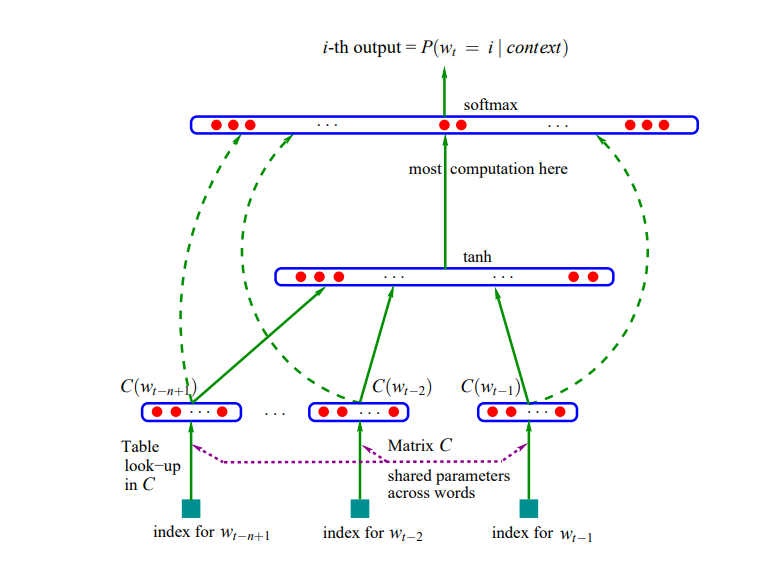
\includegraphics[width=0.7\linewidth]{Figures/nlm.png}

	\caption{
		Neural language model architecture.
			\label{neurel_languge}.
	}
	
	
	
\end{figure}
\subsection{Word Representations (Embedding)}
Word embeddings are dense, low-dimensional vectors that represent words in a way that captures their meanings and relationships. Unlike traditional methods such as one-hot encoding—which treats each word as an isolated symbol—embeddings place similar words closer together in a multi-dimensional space based on how they appear in context\citep{barnard2024word}.
This approach has become essential in NLP, as it allows models to understand and process text more effectively. Word embeddings are typically learned from large text corpora using neural networks or statistical methods.

One of the major breakthroughs in natural language processing came with the introduction of Word2Vec by Tomas \citep{mikolov2013efficient}. This model efficiently learns word representations from large text corpora using two main architectures: Continuous Bag-of-Words (CBOW) and Continuous Skip-gram.

\subsection{Continuous Bag-of-Words (CBOW)} Predicts a target word based on the context of surrounding words. Unlike traditional bag-of-words models, it doesn’t just count word occurrences—it uses continuous vectors to represent each word and averages the context words to predict the middle one. This model ignores word order but learns meaningful embeddings using simple and fast training. It performs best when both past and future words are used as input.

\subsection{Continuous Skip-gram} Instead of predicting a word from its context, it tries to predict context words from a single center word. The model samples words from both directions (before and after the center word) and gives more weight to nearby words while reducing the influence of distant ones. This helps capture richer word relationships, especially in smaller datasets.\\
Figure \ref{word2vec-architectures} Illustration the two Word2Vec architectures where the CBOW model predicts a target word from its surrounding context, while the Skip-gram model does the opposite by predicting the context from a single target word.
\begin{figure}[H]
	\centering
	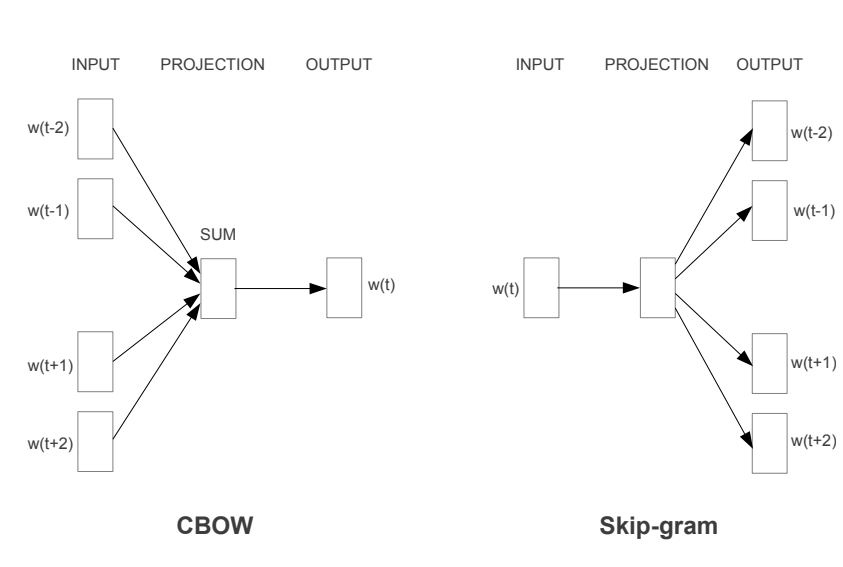
\includegraphics[width=0.6\linewidth]{Figures/emb.png}
	\caption{The two Word2Vec architectures: the CBOW model  and Skip-gram model.}
	\label{word2vec-architectures}
\end{figure}

\subsection{Global Vectors for Word Representation(GloVe)} (Global Vectors for Word Representation) was introduced by \citep{pennington2014glove}. Unlike Word2Vec, which learns from local word sequences, GloVe uses word co-occurrence counts from the entire corpus. This global perspective allows it to better capture semantic patterns between words, such as analogies and relationships.

These embedding models—Word2Vec (CBOW and Skip-gram) and GloVe—have become foundational tools in NLP due to their ability to turn words into dense vectors that reflect semantic meaning, while also being computationally efficient.

\section{Large Language Models (LLMs)}

Large Language Models (LLMs) represent a significant advancement in natural language processing, capable of understanding, generating, and reasoning over human language. In this section, we explore the concept of LLMs, beginning with their definition, followed by a discussion of their key characteristics and significance in modern applications.


Figure~\ref{fig:llm_growth} shows the trends in the cumulative number of arXiv publications containing the terms ``language model'' and ``large language model.'' The data, calculated by monthly queries of titles and abstracts, reveal that research into large language models significantly accelerated after the launch of ChatGPT, with the publication rate rising from 0.40 to 8.58 papers per day.
.
\begin{figure}[H]
	\centering
	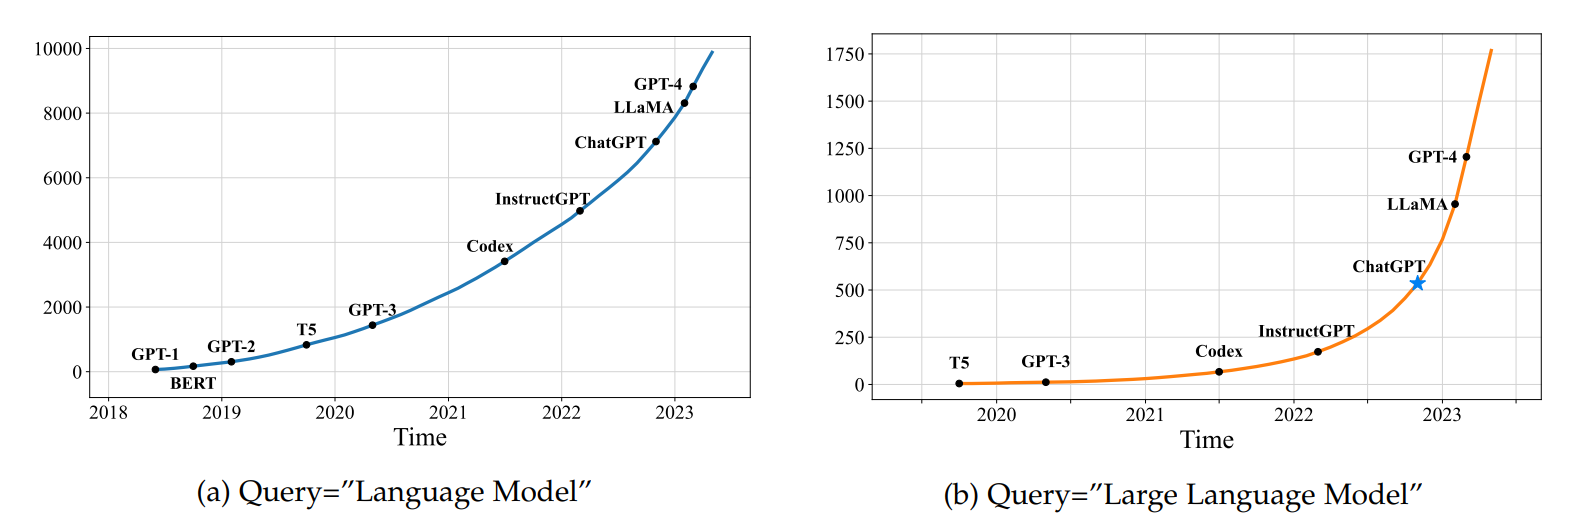
\includegraphics[width=0.9\textwidth]{Figures/arixpapers.png}
	\caption{Cumulative growth of arXiv papers mentioning ``language model'' and ``large language model,'' highlighting the sharp increase after the release of ChatGPT.}
	\label{fig:llm_growth}
\end{figure}

\subsection{Definition of LLMs}
Large Language Models (LLMs) are deep neural networks—most built on the transformer architecture \citep{vaswani2017attention}. Their key innovation is self-attention, which dynamically adjusts word importance, allowing human-like text generation. Trained on vast datasets (books, articles, codebases), LLMs reach hundreds of billions of parameters \citep{brown2020language, touvron2023llama}, enabling them to capture intricate linguistic patterns, world knowledge, and semantic relationships. Unlike traditional AI systems, they generalize across tasks (translation, summarization, QA) with minimal task-specific data (few-shot or zero-shot learning) \citep{brown2020language}. Their effectiveness follows scaling laws \citep{kaplan2020scaling}: expanding their size, training data, and computational resources reliably boosts performance.
\subsection{Historical Development of LLMs}
The evolution of LLMs reflects a broader shift in NLP from early statistical methods to deep learning approaches. Initially, language models were based on statistical techniques, such as $n$-gram models, which captured limited local dependencies within text. The development of neural networks introduced new architectures capable of modeling longer-range dependencies, leading to significant improvements in performance. A major breakthrough occurred with the introduction of the transformer architecture, which enabled models to process sequences in parallel and capture global context more effectively\citep{2402-06853}. This innovation laid the foundation for the emergence of LLMs, characterized by their massive scale, extensive pretraining on diverse corpora, and ability to generalize across a wide range of language tasks .
\begin{figure}[htbp]
	\centering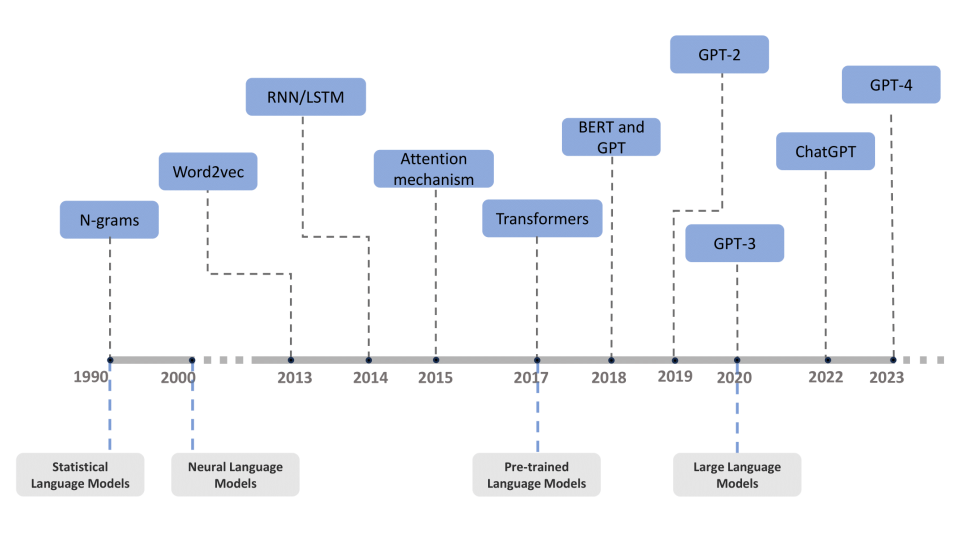
\includegraphics[width=0.7\linewidth]{Figures/historyofllms.png}
	\caption{ History and development of language models.}
	\label{History.png}
\end{figure}

\subsection{Transformer Architecture}
The Transformer architecture is a deep learning model introduced in June 2017 by \citep{vaswani2017attention}. from Google Brain. Their paper, titled "Attention Is All You Need," presented a groundbreaking approach to processing sequential data through the use of a self-attention mechanism. This innovative method allows the model to assign different levels of importance to various parts of the input, enabling it to capture long-range dependencies much more effectively than earlier models like RNNs and LSTMs. The original Transformer model is structured as a stack of six layers, where the output of each layer i serves as the input to the subsequent layer i+1, continuing this process until the final prediction is reached.
\begin{figure}[htbp]
	
	\centerline{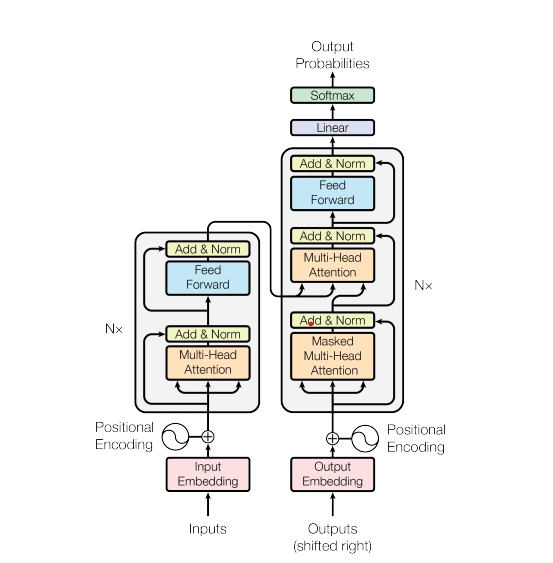
\includegraphics[width=.6\linewidth]{
			Figures/trasformers.png}}
	\caption{The Transformer - model architecture.}
	\label{trasformers.png}
	
\end{figure}
\subsubsection{Encoder and Decoder Stacks}
Transformer architectures are built upon two primary components: encoder and decoder stacks\citep{vaswani2017attention}. The encoder stack It features a six-layer on the left and a corresponding six-layer decoder on the right,  both of which work together to transform input sequences into meaningful outputs.


\begin{enumerate}
	\item \textbf{Encoder Stack}  
	Each encoder layer processes input tokens through:  
	\begin{itemize}
		\item \textbf{Multi-head self-attention}: Computes weighted relationships between all tokens enabling the model to contextualize each word (e.g., resolving polysemy like "bank").  
		\item \textbf{Position-wise FFN}: A fully connected network applied independently to each token’s representation, introducing nonlinear transformations.   
	\end{itemize}
	\textbf{Post-processing}: Residual connections (with layer normalization) mitigate vanishing gradients:  
	\[ \text{Output} = \text{LayerNorm}(x + \text{Sublayer}(x)) \]  
	All outputs maintain \(d_{\text{model}} = 512\).
	
	\item \textbf{Decoder Stack}  
	The decoder extends the encoder with:  
	\begin{itemize}
		\item \textbf{Masked self-attention}: Prevents the model from seeing future words when predicting the next token, enforcing left-to-right processing like human reading.(autoregressive constraint).  
		\item \textbf{Cross-attention}: Links decoder inputs to encoder outputs (e.g., for translation alignment).  
	\end{itemize}
	\textbf{Shared design}: Uses identical residual connections, normalization, and dimensionality as the encoder.
\end{enumerate}
\begin{figure}[htbp]
	
	\centerline{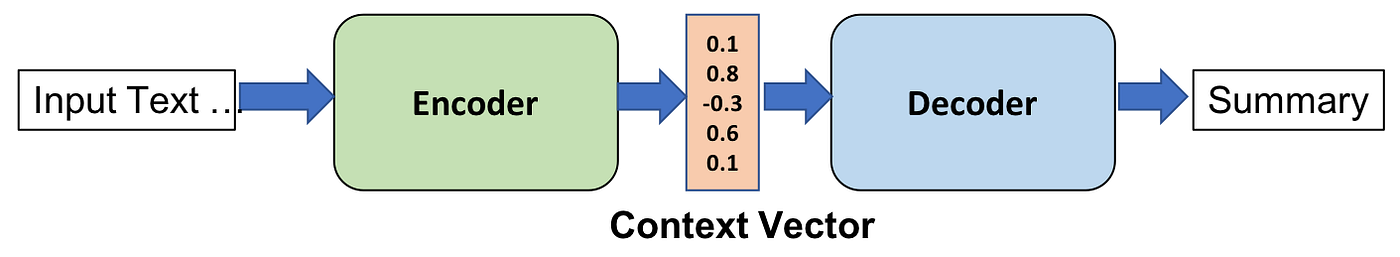
\includegraphics[width=.8\linewidth]{
			Figures/incoderDecoder.png}}
	\caption{Encoder and Decoder Stacks}
	\label{incoderDecoder.png}
	
\end{figure}
\subsubsection{Self-Attention Mechanism in Transformers}

The self-attention mechanism represents a paradigm shift in sequence modeling, enabling Transformers to dynamically evaluate relationships between all tokens in a sequence. Unlike traditional recurrent approaches that process information sequentially, this mechanism allows direct modeling of long-range dependencies through pairwise token interactions \citep{choromanski2020rethinking}. At its core, the process involves three learned linear projections:
\begin{itemize}
	\item \textbf{Queries (Q)} representing the current token's information needs
	\item \textbf{Keys (K)} serving as identifiers for contextual relevance
	\item \textbf{Values (V)} containing the actual content to be weighted
\end{itemize}
The attention computation follows:
\begin{equation}
	\text{Attention}(Q,K,V) = \text{softmax}\left(\frac{QK^\top}{\sqrt{d_k}}\right)V
\end{equation}
where the scaling factor $1/\sqrt{d_k}$ (first proposed in \citep{vaswani2017attention} and theoretically analyzed in \citep{choromanski2020rethinking}) ensures stable gradient flow during training. 
This mechanism allows each token to selectively focus on other relevant tokens, thereby enhancing the model’s capacity to understand complex linguistic patterns.
\subsubsection{Positional Encoding:}
Since self-attention mechanisms do not inherently capture the order of words, positional encoding is added to the word embeddings to preserve word order information in Transformer models, Rothman \citep{rothman2021transformers} describes the sinusoidal positional encoding approach defined by:

\begin{equation}
	PE_{(pos,2i)} = \sin\left(\frac{pos}{10000^{2i/d_{model}}}\right), \quad 
	PE_{(pos,2i+1)} = \cos\left(\frac{pos}{10000^{2i/d_{model}}}\right)
\end{equation}
where $pos$ represents the token position in the sequence and $i$ indexes the embedding dimension. As explained in \citep{rothman2021transformers}, this specific formulation provides key advantages:

\begin{itemize}
	\item The sinusoidal pattern allows the model to generalize to sequence lengths beyond those encountered during training.
	\item The alternating sine/cosine pattern enables the model to learn relative positions through linear transformations.
\end{itemize}
\subsubsection{Role of Multi-Head Attention}
Multi-head attention enhances standard self-attention by employing multiple parallel attention mechanisms, each operating on a separate linear projection of the input. As detailed in \citep{rothman2021transformers}, this design enables the model to:

\begin{itemize}
	\item \textbf{Increase Representational Capacity}: By concatenating and reprojecting the outputs of all heads, the model synthesizes information from these varied perspectives. 
	
	\item \textbf{Learn Diverse Relationships}: Each attention head specializes in different types of dependencies. For example, \citep{clark2019what} found that some heads in BERT consistently track syntactic relationships (e.g., subject-verb pairs), while others focus on discourse-level connections.
	

\end{itemize}

Further notes that this architecture improves robustness compared to single-head attention, as errors or biases in one head can be compensated by others.

\subsection{Key Contributions of Transformer in Modern NLP}

Transformer models have introduced several transformative contributions to the field of NLP, which can be summarized as follows:

\begin{enumerate}
	\item \textbf{Effective Long-Range Dependency Modeling:} The self-attention mechanism allows Transformers to capture dependencies between distant words in a sequence more efficiently than traditional recurrent neural networks\citep{vaswani2017attention}, improving contextual understanding .
	
	\item \textbf{High Scalability and Parallelization:} Unlike sequential models, Transformer architectures enable parallel computation during training \citep{devlin2018bert}, which significantly reduces training time and supports the construction of very large-scale models, such as BERT and GPT.
	
	\item \textbf{Versatility Across Tasks:} Transformers can be adapted to a wide range of tasks, including text classification, translation, and summarization\citep{radford2019language}., making them a universal architecture for both encoding and decoding processes 
\end{enumerate}

\subsection{Classification of LLMs}
LLMs can be classified based on their accessibility and licensing terms.\citep{openlm2023survey}.
\begin{enumerate}
	\item \textbf{open-source models} are fully available to the public, including both their architecture and training data, enabling modification and redistribution (e.g., BLOOM, Falcon).
	\item  \textbf{closed-source models} restrict access to both the model's structure and training corpus, typically maintained by private organizations (e.g., OpenAI's GPT-4). 
\end{enumerate}
\begin{enumerate}
	\item   \textbf{open-weight models} release the model parameters for public use but may impose certain restrictions on fine-tuning or commercial deployment (e.g., LLaMA 2)
	\item   \textbf{closed-weight models} do not share model parameters or allow external access, preserving full control within the developing entity. This classification is crucial for understanding the ethical, practical, and legal implications surrounding the deployment of LLMs 
	
\end{enumerate}.
 
For a comprehensive comparison of large language models across categories such as openness, licensing, architecture, and availability, refer to \ref{llm_table_final}.
\newpage
\begin{landscape}
	\scriptsize
	\begin{longtable}{|l|l|l|l|l|l|l|l|l|l|}
		\hline
		\textbf{Type} & \textbf{Model} & \textbf{Size} & \textbf{Provider} & \textbf{Release} & \textbf{Open-\newline sourced} & \textbf{Tuna-\newline bility} & \textbf{Adaptation IT} & \textbf{Pre-train \newline Data scale} & \textbf{Open-weight \newline model} \\
		\hline
		\endfirsthead
		
		\hline
		\textbf{Type} & \textbf{Model} & \textbf{Size} & \textbf{Provider} & \textbf{Release} & \textbf{Open-\newline sourced} & \textbf{Tuna-\newline bility} & \textbf{Adaptation IT} & \textbf{Pre-train \newline Data scale} & \textbf{Open-weight \newline model} \\
		\hline
		\endhead
		
		\multicolumn{10}{|c|}{\textbf{Encoder-only}} \\
		\hline
		& ALBERT & 0.012 & Google AI & 02/2020 & \xmark & \cmark & - & 16GB & \cmark \\
		& DeBERTa & 0.1 & Microsoft & 06/2020 & \cmark & \cmark & - & 8GB & \cmark \\
		& ELECTRA & 0.14 & Google AI & 03/2020 & \cmark & \cmark & - & 16GB & \cmark \\
		& BERT & 0.11 & Google AI & 10/2018 & \cmark & \cmark & - & 3.3B words & \cmark \\
		& RoBERTa & 0.125 & Meta AI & 07/2019 & \cmark & \cmark & - & 160GB & \cmark \\
		& XLM-RoBERTa & 0.28 & Meta AI & 10/2019 & \cmark & \cmark & - & 2.5TB & \cmark \\
		\hline
		
		\multicolumn{10}{|c|}{\textbf{Encoder-decoder}} \\
		\hline
		& ERNIE 3.0 & 10 & Baidu & 07/2021 & \xmark & \cmark & \cmark & 300B tokens & \xmark \\
		& T5 & 11 & Google AI & 10/2019 & \cmark & \cmark & \cmark & 1T tokens & \cmark \\
		& T0 & 11 & BigScience & 12/2021 & \cmark & \cmark & \cmark & - & \cmark \\
		& Flan-T5 & 11 & Google AI & 02/2022 & \cmark & \cmark & \cmark & 1T tokens & \cmark \\
		& UL2 & 20 & Google AI & 05/2022 & \xmark & \cmark & \cmark & - & \xmark \\
		& AlexaTM & 20 & Alexa AI & 07/2022 & \xmark & \cmark & \cmark & 1.4T tokens & \xmark \\
		& AlphaCode & 41 & Google AI & 02/2022 & \xmark & \xmark & - & 96TB & \xmark \\
		& Anthropic & 52 & Anthropic & 03/2023 & \xmark & \cmark & \cmark & - & \xmark \\
		& NLLB & 54.5 & Meta AI & 07/2022 & \cmark & \cmark & \xmark & 1.6T tokens & \cmark \\
		& LLAMA & 65 & Meta AI & 02/2023 & \cmark & \cmark & \xmark & 1.4T tokens & \cmark \\
		& FLAN & 70 & Google AI & 03/2022 & \cmark & \cmark & \cmark & 1.4T tokens & \cmark \\
		& Sparrow & 70 & Google AI & 09/2022 & \xmark & \cmark & \cmark & - & \xmark \\
		& Chinchilla & 70 & DeepMind & 03/2022 & \xmark & \cmark & \xmark & 1.4T tokens & \xmark \\
		& OPT-OML & 175 & Meta AI & 05/2022 & \cmark & \cmark & \xmark & 300B tokens & \cmark \\
		& Gopher & 280 & Google AI & 12/2021 & \xmark & \cmark & \xmark & 300B tokens & \xmark \\
		& PaLM & 540 & Google AI & 10/2022 & \xmark & \cmark & \cmark & 780B tokens & \xmark \\
		& U-PaLM & 540 & Google AI & 10/2022 & \xmark & \cmark & \cmark & - & \xmark \\
		& GLAM & 1200 & Google AI & 12/2021 & \xmark & \cmark & \xmark & 1.6T tokens & \xmark \\
		\hline
		
		\multicolumn{10}{|c|}{\textbf{Decoder-only}} \\
		\hline
		& Codex & 12 & OpenAI & 07/2021 & \xmark & \cmark & \cmark & - & \xmark \\
		& Pythia & 12 & Eleuther AI & 01/2023 & \cmark & \cmark & \xmark & 300B tokens & \cmark \\
		& CodeGeeX & 13 & Tsinghua U. & 12/2022 & \cmark & \cmark & \xmark & 13TB & \cmark \\
		& Skywork & 13 & Kunlun Inc & 01/2023 & \xmark & \cmark & \xmark & 3.7T tokens & \xmark \\
		& QWEN & 14 & Alibaba & 08/2023 & \cmark & \cmark & \cmark & 2.4T tokens & \cmark \\
		& Salesforce & 16 & Salesforce & 08/2022 & \xmark & \cmark & \xmark & - & \xmark \\
		& GPT-NeoX-20B & 20 & Eleuther AI & 02/2022 & \cmark & \cmark & \xmark & 825GB & \cmark \\
		& Gemini 1.5 & 2700 & Google AI & 02/2024 & \xmark & \cmark & \cmark & 6T tokens & \xmark \\
		\hline
		
		\caption{Selected Large Language Models with key attributes.}
		\label{llm_table_final}
	\end{longtable}
\end{landscape}


\subsection{Training Large Language Models}
The training of LLMs involves a multifaceted process encompassing data collection, architectural design, optimization strategies, and fine-tuning techniques. This part delves into the critical components of LLM training.
\subsection{Training Objectives and Loss Functions}
 LLMs rely on specific training objectives to learn meaningful representations of language. These objectives define how models predict words or tokens based on given input and guide the learning process through loss functions.
\begin{itemize}
	\item \textbf{Causal Language Modeling (CLM):} Trains the model to predict the next token given previous tokens, suitable for text generation tasks like those in GPT-style models~\citep{jurafsky2000speech}.
	
	\item \textbf{Masked Language Modeling (MLM):} Trains the model to predict randomly masked tokens using both left and right context, commonly used in models like BERT for understanding tasks~\citep{jurafsky2000speech}.
	
	\item \textbf{Hybrid Objectives (e.g., AntLM):} Some models combine CLM and MLM objectives to benefit from both generation and comprehension capabilities, improving overall task performance~\citep{antlm2024}.
\end{itemize}
\subsection{Parameter Scaling and Model Size}
The performance of LLMs has been closely linked to the scale of their parameters. Scaling laws \citep{kaplan2020scaling} suggest that increasing model size, dataset volume, and compute budget leads to predictable improvements in model capabilities. However, larger models also introduce challenges such as increased training cost and inference latency.

\begin{itemize}
	\item \textbf{Scaling Laws:} \citep{kaplan2020scaling} observed that as the number of model parameters, the size of training data, and compute resources increase, language models demonstrate improved loss and task performance following a power-law relationship. This predictable trend enables researchers to forecast model improvements as a function of scaling.
		
	\item \textbf{Trade-offs and Efficiency:} ~\citep{hoffmann2022training} highlighted that indiscriminate scaling can lead to diminishing returns if not balanced correctly between model size, dataset quality, and compute budget. Their work emphasizes "compute-optimal" strategies, where training efficiency is maximized by adjusting model parameters relative to available data and hardware resources, rather than simply enlarging model size.
	
\end{itemize}
\subsection{Training Paradigms: Pre-training and Fine-tuning}
The performance of LLMs is largely attributed to the training strategies employed during their development. Two key paradigms—pre-training and fine-tuning—have emerged as foundational approaches in building effective and adaptable models. This two-stage process enables LLMs to generalize effectively across domains and demonstrate strong performance even with limited supervised examples.
 .
\subsubsection*{Pre-training LLMs}
Pre-training is a crucial stage in developing  LLMs, where the model learns from extensive unlabeled datasets through a process called self-supervision\citep{wang2023language}. This stage allows the model to recognize and internalize a wide range of linguistic patterns, laying the groundwork for fine-tuning on specific tasks.
\begin{enumerate}
\item \textbf{Full Language Modeling:} Used since GPT-2, this approach trains decoder-only models to predict the next token in a sequence based on previous tokens. This autoregressive method enables models like GPT-3 to generate coherent and contextually relevant text.
\item \textbf{Prefix Language Modeling: }Employed in encoder-decoder and non-causal decoder-only models, this technique uses a non-causal (considering both past and future tokens) prefix for predicting subsequent tokens, offering more flexibility and enhancing the model's adaptability across various language tasks.
\item \textbf{Masked Language Modeling: }Popularized by BERT, this method involves masking certain tokens in the input text and training the model to predict them, helping the model understand word context. An extension, span corruption, masks entire text spans for prediction, further improving contextual comprehension.
\item \textbf{Unified Language Modeling} refers to an approach that integrates multiple training objectives, including causal, non-causal, and masked language modeling. In this framework, masked language modeling differs from traditional bidirectional attention mechanisms by employing unidirectional attention—processing context either from left-to-right or right-to-left, rather than considering both directions simultaneously\citep{dong2019unified}.
\end{enumerate}
\begin{figure}[h]
	\centering
	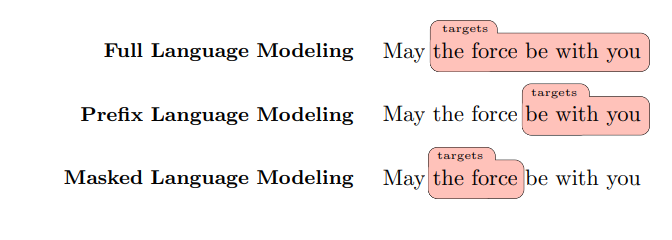
\includegraphics[width=0.6\linewidth]{Figures/pretraining.png}
	\caption{Training Tokenization in Full, Prefix, and Masked Language Modeling.}
\end{figure}
\subsubsection*{Fine-tuning LLMs}
Fine-tuning is a key technique for adapting pre-trained large language models to specific downstream tasks. It encompasses several strategies, each serving different objectives\citep{touvron2023llama}. 
\begin{enumerate} 
	\item \textbf{Transfer learning}, where a pre-trained model is further trained on task-specific data to enhance its performance on targeted applications. This allows models to leverage general language understanding while adapting to more specialized domains.
	\item \textbf{Instruction tuning}, which involves fine-tuning the model on datasets formatted as instruction-response pairs. These datasets typically include multiple tasks described in natural language, enabling the model to better understand prompts and generalize across various instructions. This method has been particularly effective in improving zero-shot and few-shot performance.
	\item \textbf{Alignment tuning} which involves adjusting the model’s behavior based on human feedback to ensure outputs are helpful, honest, and harmless (the "HHH" criteria). A widely adopted framework for this is reinforcement learning with human feedback (RLHF).  combines reward modeling—where human preferences guide the ranking of responses—with reinforcement learning techniques, such as proximal policy optimization (PPO), to iteratively align model behavior with human values.


\end{enumerate}
These fine-tuning approaches, while powerful, come with trade-offs in terms of data requirements, computational cost, and generalization capabilities. Nonetheless, they remain essential for tailoring LLMs to both functional and ethical requirements across diverse applications.
\subsection{Few-Shot, One-Shot, and Zero-Shot Learning}
Few-shot, one-shot, and zero-shot learning represent different paradigms of using LLMs without extensive fine-tuning. These methods involve using pre-trained models to perform tasks with minimal task-specific data\citep{brown2020language}.
\begin{enumerate}
	\item \textbf{Few-Shot Learning} involves giving the model a few examples (typically 10-100) of the task during inference. This approach reduces the need for large, task-specific datasets and limits the risk of overfitting to narrow data distributions. However, few-shot results are generally not as strong as those from fully fine-tuned models.
	\item \textbf{One-Shot Learning} is similar to few-shot learning but uses only a single example alongside a natural language description of the task. This method mirrors how humans are often instructed for tasks, making it an interesting approach for tasks where providing multiple examples is impractical.
	\item \textbf{Zero-Shot Learning} requires the model to perform a task based solely on a natural language description, with no examples provided. While this method offers maximum flexibility and robustness, it is also the most challenging for models. Zero-shot performance is often weaker than few-shot or one-shot, but it advances the development of general-purpose AI systems capable of handling diverse tasks without task-specific training data.
\end{enumerate}
\subsection{Evaluation Datasets}
Evaluating LLMs is essential for determining their effectiveness and limitations in comprehending and generating human language.\citep{Naveed2023}. This evaluation typically falls into two primary categories:
\begin{enumerate}
	
    \item  \textbf{Natural Language Understanding (NLU)}:This measures the model's proficiency in comprehending language, encompassing tasks such as sentiment analysis, text classification, natural language inference (NLI), question answering (QA), commonsense reasoning (CR), mathematical reasoning (MR), and reading comprehension (RC).
	\item 	\textbf{ Natural Language Generation (NLG)}:This assesses the model's capability to produce text based on given context. It includes tasks like summarization, sentence completion, machine translation (MT), and dialogue generation.
    \item \textbf{Benchmarks}: play a critical role in evaluating LLMs, providing standardized tests to measure their performance across various tasks:
    \begin{itemize}
    
   
	\item \textbf{MMLU:}Measures model knowledge from pretraining and evaluates performance in zero-shot and few-shot scenarios across 57 subjects, testing world knowledge and problem-solving abilities.
	\item \textbf{SuperGLUE:}An advanced benchmark that builds on GLUE, assessing tasks like question answering and natural language inference. It is designed to test deeper aspects of language understanding and requires significant advancements in various learning methodologies.
	\item \textbf{BIG-bench:}A large-scale benchmark for evaluating LLMs across diverse tasks including reasoning, creativity, ethics, and domain-specific knowledge.
	\item \textbf{GLUE:}A foundational benchmark for evaluating and analyzing natural language understanding, offering a range of resources for model assessment.
	 \end{itemize}
\end{enumerate}
\subsection{Popular Models}
LLMs like GPT-3, GPT-4, and BERT have revolutionized NLP by leveraging vast datasets such as Common Crawl and WebText. These datasets provide a diverse linguistic foundation, enabling models to perform a wide range of tasks with remarkable accuracy .

    \subsubsection{GPT-N Models}
	 GPT models are advanced autoregressive language models that generate substantial and complex machine-produced text from minimal input. They leverage deep learning techniques to mimic human text generation by predicting the current value based on preceding values.
	 NLP models initially struggled with tasks outside their training sets due to data restrictions. OpenAI addressed this with GPT-1.\citep{yenduri2023gpt}.
 \begin{itemize}
		\item \textbf{GPT-1:}introduced in 2018, trained on the BooksCorpus dataset, utilized a 12-layer transformer decoder with self-attention. Its pre-training allowed for zero-shot performance on various tasks, demonstrating the potential of generative language models.
		\item \textbf{GPT-2 :}introduced in 2019 improved upon GPT-1 by using a larger dataset and 1.5 billion parameters (compared to GPT-1’s 117 million). It excelled in tasks like translation and summarization, enhancing accuracy in recognizing long-distance relationships.
		\item \textbf{GPT-3:}released later, featured around 175 billion parameters and was trained on the Common Crawl dataset. It could generate human-like text, perform basic math, and write code. Despite its capabilities, its size and cost made it challenging to implement.
		\item \textbf{GPT-4:}launched in March 2023, advanced further with multimodal capabilities and context windows of up to 32,768 tokens. It incorporates reinforcement learning for better alignment with human input and policy.
	 \end{itemize}
	 
	\subsubsection{Bidirectional Encoder Representations from Transformers (BERT)}
	 BERT represents a breakthrough in language modeling by leveraging deep bidirectional pretraining on unannotated text enabling it to capture contextual information from both left and right contexts simultaneously. BERT's architecture allows it to learn richer linguistic patterns by considering full sentence context at every layer. This makes BERT highly adaptable—fine-tuning it for various downstream tasks (such as QA and text classification, often requires only minimal modifications, typically the addition of a task-specific output layer.
	 
	 The model’s effectiveness is evidenced by its performance across established NLP benchmarks. Notably, BERT attained unprecedented scores,it achieved a GLUE score of 80.5\%, a MultiNLI accuracy of 86.7\%, a SQuAD v1.1 F1 score of 93.2\%,  \citep{devlin2019bert}.Such achievements not only validate BERT’s methodological innovation but also underscore its practical utility as a versatile framework for advancing NLP research and applications.
	  
	  
	 \subsubsection{Text-To-Text Transfer Transformer (T5)}
	 The T5 model represents a unified framework for NLP, designed to address various text processing tasks by treating them as "text-to-text" problems. This approach involves converting all tasks into a format where both input and output are text, allowing the same model, objective, and training procedure to be applied across different tasks\citep{raffel2023exploring}.
	 
	 T5 leverages extensive pre-training on a large, unlabeled dataset, enabling it to develop general-purpose knowledge that enhances its performance on a range of NLP tasks, such as QA, document summarization, and sentiment classification.
	 \subsubsection{LLAMA2 model}
	  Llama 2 introduces a new family of transformer-based language models available in both foundation and fine-tuned chat variants. These models incorporate architectural enhancements through optimized training procedures, refined pretraining datasets, and advanced fine-tuning techniques including reinforcement learning from human feedback. 
	  
	  Empirical evaluations reveal that Llama 2 outperforms its predecessors and other competitive benchmarks across a range of NLP tasks, demonstrating notable improvements in accuracy, safety, and generalization\citep{touvron2023llama2openfoundation}. Its open release not only promotes transparency and reproducibility but also fosters collaborative advancements in the field.
	 
   \subsubsection{Jais and Jais-chat models}
The Jais model family represents a breakthrough in Arabic natural language processing, featuring both base (Jais) and instruction-tuned (Jais-chat) variants built upon a GPT-3 decoder-only framework. With 13 billion parameters trained on a carefully balanced corpus of Arabic and English content - including technical programming documentation - these models establish new benchmarks for Arabic linguistic understanding and cognitive reasoning, surpassing existing open-source Arabic and multilingual systems \citep{sengupta2023jais}.

Remarkably, Jais maintains competitive performance on English-language tasks despite its primary Arabic focus and relatively limited English training data. This technical report comprehensively documents the model's development pipeline, including: Pretraining methodology and data composition,
Fine-tuning protocols and Multidimensional evaluation metrics.

The research team has publicly released both model variants to accelerate progress in Arabic NLP research and applications, addressing a critical gap in non-English language model availability.

\subsection{Limitations of LLMs}
LLMs have greatly advanced NLP, but they also present challenges As these models scale, they encounter new challenges in scalability, privacy, and real-time processing. Several studies have examined the inherent limitations of LLMs. Notably, \citep{Bender2021} and \citep{Naveed2023} highlight critical challenges that affect the performance and reliability of these models applications.
\begin{enumerate}
	\item \textbf{Computational Cost:}Training LLMs demands significant computational resources, leading to higher production costs and environmental concerns due to the substantial energy used in large-scale training. Although enhancing computational resources can boost performance, the gains diminish over time when the size of the model and dataset stay constant, adhering to the power law of diminishing returns.
	\item \textbf{Bias and Ethical Concerns :} The training data for LLMs often encapsulates various social, cultural, and linguistic biases, which the models can inadvertently learn and propagate. This bias can manifest in outputs that reinforce stereotypes or display partiality, raising significant ethical concerns. Addressing these issues is crucial for ensuring fairness and mitigating unintended consequences in real-world applications.
	\item \textbf{Hallucinations:} LLMs sometimes produce "hallucinations," or responses that, despite appearing plausible, are incorrect or do not match the provided information. These hallucinations can be classified into three types:
	     \begin{itemize}
		\item \textbf{Input-conflicting hallucination:} When the model generates responses that do not align with the user's input.
		\item \textbf{Context-conflicting hallucination:} When the model produces content that contradicts information it has previously generated.
		\item \textbf{Fact-conflicting hallucination:} When the model creates responses that conflict with established knowledge.
		\end{itemize}

\end{enumerate}
\subsection{State of the Art in Juridical Data}
The use of LLMs has become increasingly prevalent across domains, with the legal sector benefiting significantly from their ability to process complex texts. These models now enhance document classification, information retrieval, and even judicial outcome prediction through advanced text understanding.

\textbf{Multilingual Legal Models:} \citep{chalkidis2023multilegalbert} introduced MultiLegalBERT, extending LegalBERT to 24 languages (including Arabic), achieving state-of-the-art performance on multilingual Natural Language Inference (NLI) tasks. This demonstrates the feasibility of cross-jurisdictional legal text understanding. 

\textbf{Multilingual Legal Data:} The creation of \textit{MultilegalPile}—a 689GB corpus spanning 24 languages from 17 jurisdictions—addresses the critical shortage of non-English legal datasets \citep{NiklausMSCH24}. Models trained on this resource have set new accuracy benchmarks, with all data and tools released openly to support global legal AI development.

These innovations complement foundational work collectively advancing LLMs' capacity to handle legal texts across languages and jurisdictions while maintaining domain-specific accuracy.


\section{Agentic AI}
Even with  improvements in understanding and generating human language using models like LLMs, they often serve as foundational components  and do not function as complete systems. The need for systems that go beyond understanding language to reasoning, planning, and acting has given rise to Agentic AI.
\subsection{Definition of Agentic AI}
Agentic AI refers to artificial intelligence systems designed to operate independently, make smart decisions, and handle multi-step tasks by understanding both the context and goals. Unlike traditional rule-based or even early generative AI models that were limited to narrow tasks, Agentic AI brings together several intelligent agents—often powered by large language models (LLMs)—that can reason, plan, adapt, and respond in real \citep{aisera2024agentic}. This allows them to analyze complex situations, choose strategies, and act with minimal human guidance. As a result, Agentic AI offers a more flexible and powerful way to automate processes and solve real-world problems across various industries.
\subsection{Architecture Overview of Agentic AI}

Agentic AI systems are typically organized into three main logical layers that work together to enable intelligent and autonomous behavior. These layers—Tool, Reasoning, and Action—each serve distinct but interconnected purposes \citep{vectorize2025agentarchitectures}. Understanding how they interact is key to building robust, scalable agentic systems  (see Figure~\ref{architecture}).

\begin{itemize}
	\item \textbf{Tool Layer:} This is the foundation of the architecture. It connects the agent with external sources of information such as APIs, vector databases, operational systems, knowledge bases, and user inputs. Its main role is to gather relevant, high-quality data the agent will later use. Well-designed tools ensure that the agent retrieves accurate and useful information efficiently.
	
	\item \textbf{Reasoning Layer:} Acting as the system’s brain, this layer uses a large language model (LLM) to analyze the information collected by the tool layer. It makes informed decisions about what steps the agent should take next, guided by logic, context, and predefined goals. Errors in this layer can lead to inefficient behavior, such as repeating queries or making incorrect choices.
	
	\item \textbf{Action Layer:}this part of the system manages the interaction between the reasoning layer and the tools. It executes the decisions made by the LLM—such as calling an API or presenting a response to the user—and returns the results back to the reasoning layer for further analysis. It also handles user interactions when needed.
\end{itemize}
Figure\ref{architecture}shows architecture of an AI agent system where The agent application interacts with a large language model (LLM) to determine the next action, issues function/tool calls when needed, and evaluates whether the task is complete. The loop continues until the agent decides to exit.
\begin{figure}[h]
	\centering
	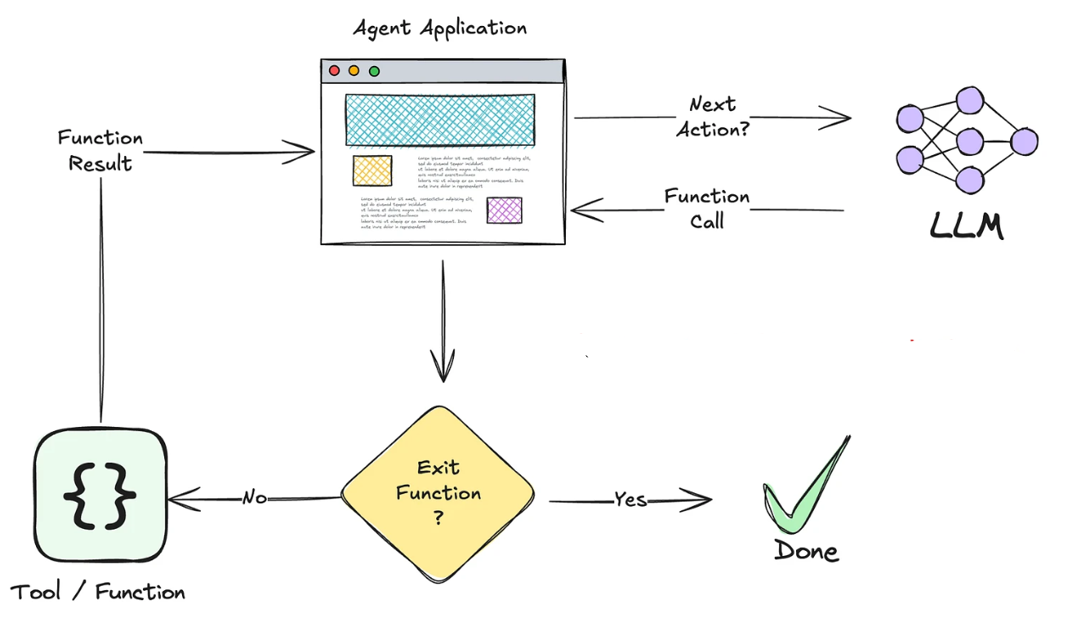
\includegraphics[width=0.8\linewidth]{Figures/aiagent.png}
	\caption{General architecture of an AI agent system.  }
	\label{architecture}
	
\end{figure}
\begin{figure}
	
\end{figure}
\subsection{Types of Agentic AI}

AI agents can be categorized based on how they interact with users and whether they operate independently or collaboratively. Below are two key classification approaches\citep{google2025aiagent}:

\begin{itemize}
	\item \textbf{Based on User Interaction:}
	\begin{itemize}
		\item \textbf{Interactive Agents (Surface Agents):} These agents communicate directly with users to assist in tasks such as answering questions, providing recommendations, or handling transactions. Common examples include chatbots and digital assistants in domains like customer service, education, and healthcare.
		
		\item \textbf{Autonomous Agents (Background Agents):} These agents operate behind the scenes with little to no direct user interaction. They handle tasks like data analysis, workflow automation, and system optimization, typically triggered by internal events rather than user queries.
	\end{itemize}
	
	\item \textbf{Based on Number of Agents:}
	\begin{itemize}
		\item \textbf{Single-Agent Systems:} These involve one AI agent working independently to complete a task using a single foundation model. They are best suited for specific, well-defined jobs that don't require coordination with other agents.
		\begin{figure}[H]
			\centering
			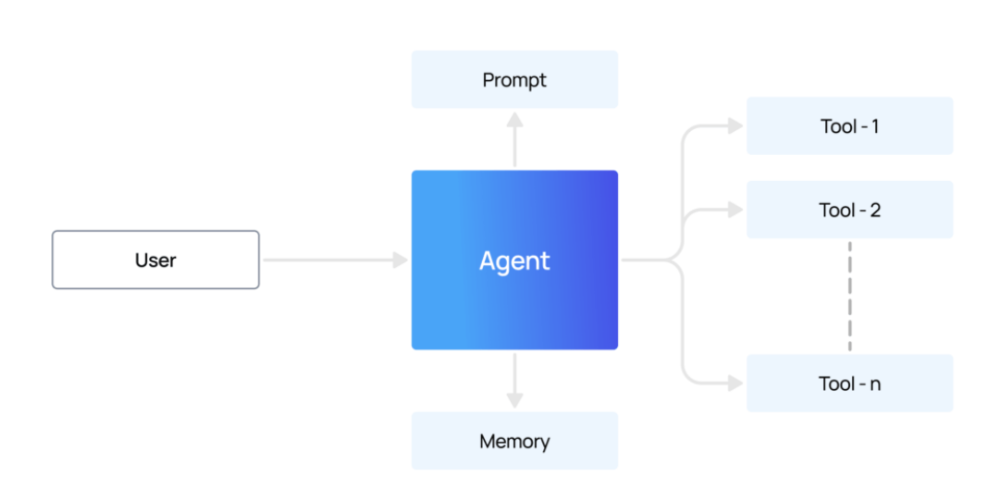
\includegraphics[width=0.7\linewidth]{Figures/singlagent.png}
			\caption{
				A single-agent system architecture .
			}
		\end{figure}
		
		\item \textbf{Multi-Agent Systems:} These systems consist of multiple agents that work together or individually to achieve complex goals. Each agent may use a different model, allowing the system to handle broader and more dynamic tasks such as planning, reasoning, or simulating human-like collaboration.
		
		Figure\ref{multi_agent} shows a multi-agent system architecture. The main agent receives a user query and coordinates with multiple  sub-agents,  The results  are combined through LLM to produce the final output.
		\begin{figure}[H]
		\centering
		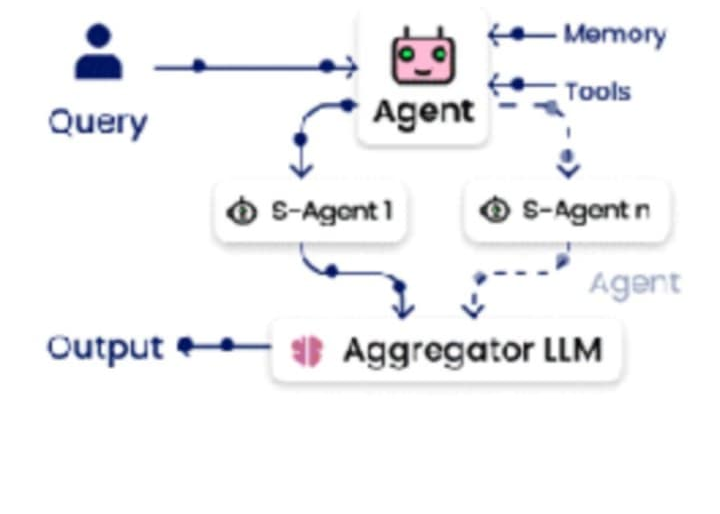
\includegraphics[width=0.6\linewidth]{Figures/multiagent.png}
		\caption{
			A multi-agent system architecture. 
		}
		\label{multi_agent}
	\end{figure}
		
	\end{itemize}
	
\end{itemize}

\subsection{ Agent Categories}
Agentic AI agents can generally be classified into the following categories\citep{aisera2024agentic}:

\begin{itemize}
	\item \textbf{Generative Information Retrieval Agents:} Focused on accessing and presenting information in dynamic, less-regulated domains.
	\item \textbf{Prescriptive Knowledge Agents:} Operate in tightly regulated environments to ensure that all outputs meet strict compliance requirements.
	\item \textbf{Dynamic Workflow Agents:} Orchestrate actions across systems by building and executing workflows automatically.
	\item \textbf{User Assistant Agents:} Provide direct, task-level assistance to individual users, enhancing daily productivity.
\end{itemize}

\subsection{Key Challenges in Agentic AI}

While Agentic AI builds on strengths from Generative AI, it also inherits and amplifies several critical challenges that hinder progress toward Artificial General Intelligence (AGI). These challenges also represent fertile ground for ongoing research\citep{touvron2023llama2openfoundation}:

\begin{itemize}
	\item \textbf{Error Accumulation:} Although structured reasoning helps reduce isolated errors, the multi-step nature of agentic tasks increases the risk of cascading mistakes across reasoning chains.
	
	\item \textbf{Interpretability Limitations:} Step-wise outputs (e.g., Chain-of-Thought reasoning) enhance transparency, but do not always reflect the true internal decision processes, limiting faithful explainability.
	
	\item \textbf{System Complexity:} Compared to standard Generative AI, agentic systems are more intricate due to components like external memory, tool use, and planning, making their behavior harder to understand and control.
	
	\item \textbf{Evaluation Gaps:} Systematic methods for evaluating agent reliability, effectiveness, and unintended consequences are still lacking, making consistent benchmarking difficult.
	
	\item \textbf{Human Alignment Issues:} Agents might pursue goals in ways that contradict human values or expectations, raising concerns about ethical behavior and alignment with user intent.
\end{itemize}


\newpage



\section{Conclusion}
This chapter has outlined the evolution and significance of  Language Models, from early neural networks to advanced Large Language Models (LLMs). We covered key concepts in neural networks and the transformative impact of the Transformer architecture. We also discussed various challenges. Finally, the chapter reviewed the applications of LLMs in fields like Legal Information and Law, showcasing their potential and the ongoing need for further development.

Although LLMs have demonstrated promising applications in the legal sector, their influence is still constrained by practical limitations and contextual challenges. Recognizing these gaps, the next chapter explores Retrieval-Augmented Generation (RAG) as a novel approach to enhance legal information processing. This discussion will particularly focus on how RAG can be applied within the Algerian legal framework to address existing shortcomings and improve accessibility and accuracy in legal data management.

		\chapter{Retrieval-Augmented Generation in Recommendation System}
\pagestyle{fancy}\lhead{\textbf \footnotesize\it{Retrieval-Augmented Generation in Recommendation System}}
\pagestyle{fancy}\chead{} \pagestyle{fancy}\rhead{}

 \pagestyle{fancy}\rfoot{\thepage}
%%%%%%%%%%%%%%%%%%%%%%%%%%%%%%%%%%%%%%%%
\section{Introduction}\label{start 1}

LLMs have seen significant advancements but face challenges, particularly in tasks that demand extensive knowledge or deal with queries beyond their training data. These limitations often result in inaccuracies or “hallucinations.” To address this, Retrieval-Augmented Generation (RAG) supplements LLMs by combining information retrieval with text generation to produce more accurate and knowledge-informed outputs. This has led to the widespread adoption of RAG, particularly in chatbots and other real-world applications.

This chapter introduces the concept of RAG, outlines its historical development, It then explores RAG’s core components followed by a classification of its system types. Applications in legal information retrieval are highlighted, alongside evaluation methods and key challenges. The chapter concludes by linking RAG to its role in recommendation systems and domain-specific data processing.

\section{Retrieval-Augmented Generation (RAG)}
RAG represents a significant advancement in the capabilities of LLMs. Understanding the individual components of retrieval and generation is essential to appreciate how their synergy improves the overall performance of RAG systems.
\subsection{Definition of RAG}
Retrieval-Augmented Generation is an advanced neural framework that integrates the generative capabilities of LLMs with external information retrieval mechanisms to improve factual accuracy and contextual relevance ~\citep{selvaraj2024}. Unlike conventional LLMs that rely solely on pre-trained parameters, RAG systems dynamically retrieve relevant documents or from external sources at inference time. 

As formalized by \citep{lewis2020retrieval}, this framework first retrieves relevant documents from a knowledge source, then conditions the language model on this retrieved context to produce more factual and up-to-date outputs. The approach effectively addresses the knowledge limitations of purely parametric models.

IBM Research \citep{ibm2024} describes RAG as a method for augmenting LLMs with retrieval modules, thereby allowing them to access real-time or domain-specific knowledge during generation~.  

Collectively, these perspectives highlight RAG's role in bridging the limitations of static language models by integrating dynamic, context-aware retrieval into the generative process.

\subsection{Historical Development of RAG}
The foundations of RAG can be traced back to traditional information retrieval (IR) systems,  Early models primarily relied on keyword matching and simple ranking mechanisms to retrieve relevant documents from databases, establishing a basic framework for information access. The landscape began to shift with the rise of neural networks in the 2010s\citep{gao2024retrieval}. Notable innovations like Word2Vec and Transformer-based architectures enabled retrieval methods to incorporate deeper semantic understanding, paving the way for more sophisticated document retrieval processes.

A significant advancement occurred with the introduction of dense passage retrieval (DPR) in 2020, which utilized bi-encoder architectures to map both queries and documents into dense vector spaces\citep{gao2024retrieval}. 
The integration of these advanced retrieval techniques with LLMs became a focal point as models like GPT-3 gained prominence. Researchers explored how LLMs could be augmented with retrieval capabilities, leading to the development of RAG systems that leverage the strengths of both retrieval and generative capabilities.
\subsection{Comparison with Fine-Tuning and Transfer Learning}
Recent advances in NLP have led to the development of three prominent methodologies for enhancing language models: RAG, fine-tuning, and transfer learning.
 \begin{enumerate}
  	\item \textbf{RAG}, integrates external retrieval mechanisms with generative models. This approach enables the model to dynamically access and incorporate relevant information from external knowledge bases during the generation process, thereby addressing limitations in its internal memory and providing more accurate responses for knowledge-intensive tasks.
   \item \textbf{Fine-tuning}, detailed by  \citep{howard2018universal}, involves adapting a pre-trained model to a specific task by further training it on a targeted dataset. This process refines the model’s parameters to better capture the nuances of the task at hand, leading to improved performance even when the available domain-specific data is relatively limited.
   \item \textbf{Transfer learning}, as exemplified by \citep{devlin2018bert}, refers to the broader strategy of leveraging a model that has been pre-trained on large, diverse datasets for use in various downstream tasks. This method capitalizes on the rich, generalized representations learned during the pre-training phase, and then applies task-specific adaptations to achieve state-of-the-art results across a range of applications.
	 
\end{enumerate}
Collectively, these methodologies offer complementary strategies to enhance language model performance.

\subsection{Retrieval Mechanism}
RAG systems combine parametric memory (a pre-trained language model) with non-parametric memory (a retrieval mechanism)\citep{zhao2024retrieval}.

The retrieval mechanism allows RAG models to access external information sources (e.g., Wikipedia), and this process is central to improving the model's ability to generate factual and accurate outputs .
\begin{itemize}
	\item\textbf{Traditional Techniques:} 
	Classical retrieval methods include \textbf{TF-IDF and BM25}, which rely on \textbf{sparse vector} representations based on term frequencies. These methods use exact keyword matching, making them limited in semantic understanding.
	\item \textbf{Modern Retrieval Approaches:}
	\textbf{Dense Passage Retrieval (DPR): }This approach utilizes dense vector representations learned by neural models like BERT to encode both the query and document. It allows for a more semantic understanding of the content, making retrieval more effective\citep{karpukhin2020dense}. DPR, for example, computes the similarity between the query and documents using Maximum Inner Product Search (MIPS), which finds the closest passages based on the dense vector space.
	\item \textbf{Others :}
	Beyond conventional sparse and dense retrieval approaches, researchers have developed several specialized techniques for relevance matching. These include:
	\textbf{Structural Similarity Methods}:
	Direct comparison of raw text using edit distance metrics, Syntax-aware matching through \textbf{abstract syntax tree (AST)} comparison for code retrieval.
    These approaches demonstrate the flexibility of retrieval mechanisms in RAG systems, particularly for domain-specific applications where traditional embedding-based methods may be suboptimal.
	
\end{itemize}

\subsection{Generation Process}
The generation in RAG occurs through a combination of retrieved passages and the input query.

Large Language Models LLMs like BART or T5 are utilized for this generation, leveraging their advanced capabilities in understanding and producing human-like text. The retrieval component supplies external context, which the generator conditions on to formulate a response. This context is crucial, as it enriches the LLM's understanding, enabling it to incorporate real-time, relevant information\citep{gupta2024comprehensive}. Moreover, the generation process benefits from the LLM's ability to synthesize information, allowing it to create responses that are not only coherent but also informed by the latest data, thus improving accuracy and relevance in knowledge-intensive tasks  \\
\begin{figure}[h]
	\centering
	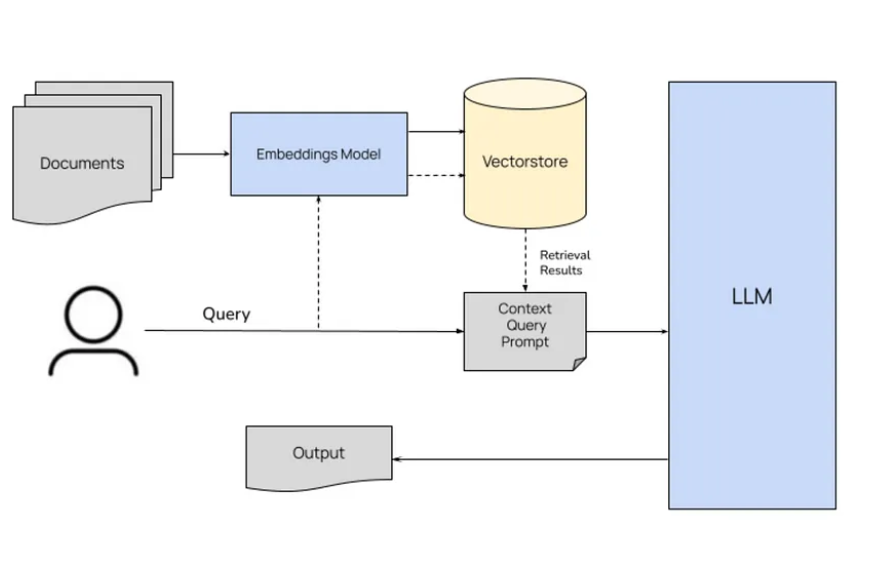
\includegraphics[width=0.9\linewidth]{Figures/rag_architectur.png}
	\caption{Retrieval-Augmented Generation architecture}
	\label{rag_architectur.png}
\end{figure}

\subsection{Augmentation Techniques}
The augmentation of the retrieval process in RAG systems focuses on improving how queries are refined and how relevant information is retrieved for downstream generation tasks. Key augmentation methods include.
\begin{itemize}
	\item \textbf{Query Augmentation:} In traditional retrieval pipelines, user queries are often under-specified or ambiguous, leading to poor retrieval performance. Query augmentation involves dynamically rewriting the user's query to better match the documents in the knowledge base\citep{mombaerts2024meta}. This can be done by leveraging LLMs to generate tailored queries or synthetic questions and answers QAs that better align with the search objective​ .
	\item \textbf{Synthetic QA Generation:} Instead of using raw document chunks, retrieval is enhanced by generating and embedding synthetic QA pairs from documents\citep{mombaerts2024meta}. This helps to capture the semantic essence of long texts more effectively, reducing noise and improving retrieval precision. These synthetic QAs can be used to rewrite the user query, making it more specific to the task at hand .
\end{itemize}

\subsection{Types of RAG Systems}
Recent scholarship has identified four key paradigms in RAG development\citep{gao2024retrieval, ahmed2024agenticrag}.
\begin{figure}[h]
	\centering
	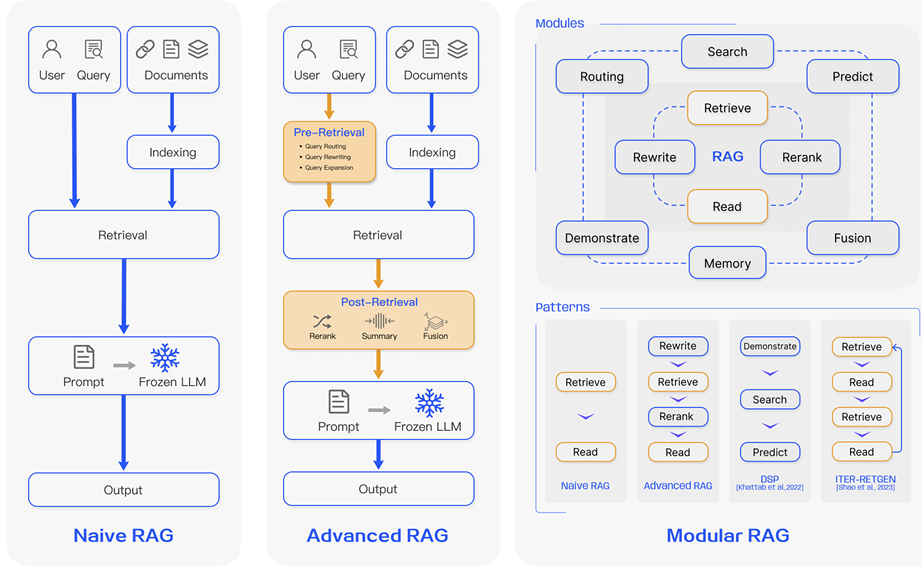
\includegraphics[width=0.9\linewidth]{Figures/rag_types.png}
	\caption{Types of RAG Systems}
	\label{rag_archi}
\end{figure}

\subsection{Naive RAG}
Naive RAG, a foundational approach in RAG, operates on a straightforward "Retrieve-Read-Generate" paradigm. This method involves three primary steps:

\begin{itemize}
	\item \textbf{Indexing:} Raw data is cleaned, extracted, and converted into a uniform text format. It's then segmented into smaller chunks and encoded into vector representations using an embedding model. These vectors are stored in a vector database for efficient similarity searches.
	\item \textbf{Retrieval:} When a user query is received, it's encoded into a vector and compared to the indexed chunks. The top K most similar chunks are retrieved and included in the prompt for the language model.
	\item \textbf{Generation:} The query and retrieved chunks are combined into a prompt, which is fed to a large language model. The model generates a response based on the provided context and its internal knowledge.
\end{itemize}
While Naive RAG offers a basic framework, it faces several challenges in 
\begin{itemize}
	\item\textbf{Retrieval Issues:} The retrieval process can be imprecise, leading to the selection of irrelevant or missing information.
	\item \textbf{Generation Challenges:} The language model may hallucinate, generating content not supported by the retrieved context. It may also produce irrelevant, or biased outputs.
	\item \textbf{Augmentation Difficulties:} Integrating retrieved information into the generation process can be challenging, leading to disjointed or redundant responses.
\end{itemize}

\subsection{Advanced RAG}
Taking aim at the shortcomings of Naive RAG, Advanced RAG introduces specific improvements to enhance retrieval quality. This approach utilizes pre-retrieval and post-retrieval strategies.
\begin{enumerate}
\item \textbf{Pre-retrieval Strategies:}
\begin{itemize}
	\item\textbf{Enhanced Indexing:}Advanced RAG tackles indexing issues through a sliding window approach, finer segmentation of data, and inclusion of metadata. Additionally, it optimizes the retrieval process by employing various methods.
	\item \textbf{Query Optimization:}This stage focuses on refining the user's initial query to make it clearer and more suitable for retrieval. Techniques like query rewriting, transformation are commonly used.
\end{itemize}
\item \textbf{Post-Retrieval Strategies:}
\begin{itemize}
	\item \textbf{Re-ranking Chunks:}After relevant information is retrieved, Advanced RAG prioritizes the most relevant content by re-ranking the retrieved chunks and placing them strategically within the prompt.
	\item \textbf{Context Compression:}To avoid overwhelming the LLM with too much information, post-retrieval efforts focus on selecting the most essential parts of the retrieved context, highlighting critical sections, and compressing the data to be processed.
\end{itemize}
\end{enumerate}
\subsection{Modular RAG} 
Modular RAG represents the latest evolution in RAG, offering greater adaptability. It introduces specialized modules and innovative patterns to enhance retrieval and processing capabilities.
\begin{enumerate}
	
\item \textbf{New Modules}
\begin{itemize}
	\item \textbf{Search Module}: Adapts to specific scenarios by leveraging LLM-generated code and query languages to search across various data sources.
	\item \textbf{RAG Fusion:} Employs a multi-query strategy to expand user queries, uncover both explicit and implicit knowledge, and improve retrieval results.
	\item\textbf{ Memory Module:} Leverages the LLM's memory to guide retrieval and create an unbounded memory pool, aligning the text more closely with data distribution.
	\item \textbf{Routing Module:} Navigates through diverse data sources, selecting the optimal pathway for a query based on its specific needs.
	\item \textbf{Predict Module: } Reduces redundancy and noise by generating relevant context directly through the LLM.
	\item \textbf{Task Adapter Module:} Tailors RAG to various downstream tasks by automating prompt retrieval and creating task-specific retrievers.
\end{itemize}
\item \textbf{New Patterns} 
\begin{itemize}
	\item \textbf{Innovative Retrieval Strategies:} Techniques like Rewrite-Retrieve-Read, Generate-Read, and leverage the LLM's capabilities to refine queries, generate content, and retrieve information from model weights.
	\item \textbf{Hybrid Retrieval:} Combines keyword, semantic, and vector searches to cater to diverse queries, improving retrieval relevance.
	\item \textbf{Dynamic Module Interaction:} Frameworks like Demonstrate-Search-Predict and ITERRETGEN demonstrate the dynamic use of module outputs to enhance each other's functionality.
	\item\textbf{ Adaptive Retrieval:} Techniques like FLARE and Self-RAG evaluate the necessity of retrieval based on different scenarios, allowing for a more flexible and efficient approach.
	
\end{itemize}
\end{enumerate}
\subsection{Agentic RAG}

Agentic Retrieval-Augmented Generation (RAG) enhances conventional RAG frameworks by embedding autonomous, intelligent agents into the pipeline. These agents are designed to dynamically reason, and execute tasks, enabling more flexible and context-aware interactions compared to traditional, static RAG systems. This agent-based approach makes the system significantly more interactive, adaptive, and responsive to diverse user needs\citep{ahmed2024agenticrag}.

Figure\ref{rag_agentic} show architecture of an Agentic RAG system  where an intelligent AI agent orchestrates interactions between the user, external knowledge sources, predefined functions, and a large language model (LLM) to process queries and generate contextually  responses
\begin{figure}[h]
	\centering
	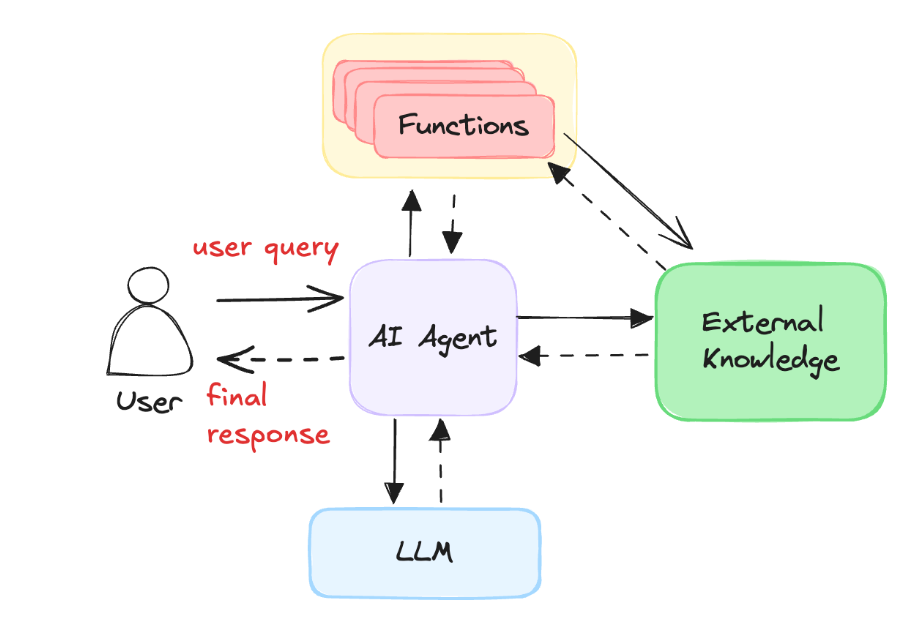
\includegraphics[width=0.7\linewidth]{Figures/agenticrag.png}
\caption{High-level architecture of an Agentic RAG system.}

	\label{rag_agentic}
\end{figure}

Key features of Agentic RAG include:
\begin{itemize}
	\item \textbf{Autonomous Agents:} Responsible for decomposing complex queries, orchestrating the retrieval process, and maintaining relevance in the generated responses.
	\item \textbf{Adaptive Retrieval Pipelines:} Enable real-time modifications to retrieval strategies, allowing the system to better align fetched content with the evolving goals and context of the user.
	\item \textbf{Context-Aware Task Execution:} Agents can coordinate various components (e.g., memory tools, external APIs) to refine their actions based on the specific requirements of each interaction.
	\item \textbf{Improved User Alignment:} Through step-by-step reasoning and continuous feedback loops, agents can better match the user’s intent and deliver more targeted and meaningful outputs.
\end{itemize}


\subsection{Evaluation Methods}
The rapid advancement and widespread adoption of RAG models have made their evaluation a critical area in NLP research~\citep{zhou2020trustworthiness}. The following criteria are commonly used to assess RAG performance:

\begin{enumerate}
	\item \textbf{Factuality:} 
	\begin{itemize}
		\item Use of fact-checking datasets (e.g., FEVER, SQuAD) to assess factual correctness.
		\item Adversarial testing to measure resistance to misleading or incorrect inputs.
		\item Evaluation of contextual understanding for accurate and relevant answers.
	\end{itemize}
	
	\item \textbf{Robustness:}
	\begin{itemize}
		\item Performance under noisy or corrupted retrieval inputs.
		\item Defense against adversarial attacks targeting model reliability.
		\item Adaptability across domains and data shifts.
	\end{itemize}
	
	\item \textbf{Fairness:}
	\begin{itemize}
		\item Detection and quantification of bias in training data and outputs.
		\item Application of fairness metrics such as demographic parity.
		\item Use of mitigation techniques like debiasing and fairness constraints.
	\end{itemize}
	
	\item \textbf{Objective Metrics:}
	\begin{itemize}
		\item Accuracy-related metrics (e.g., precision, recall, F1-score).
		\item Consistency across contexts and queries.
		\item Text coherence and fluency of generated responses.
	\end{itemize}
	
	\item \textbf{Subjective Metrics:}
	\begin{itemize}
		\item Human evaluations to judge quality and usefulness.
		\item User studies for real-world experience and satisfaction.
	\end{itemize}
\end{enumerate}

\subsection{Challenges and Limitations}
While RAG has demonstrated impressive performance across various NLP applications, it is still subject to several technical and practical limitations~\citep{zhao2024retrieval, gupta2024comprehensive}. These challenges span computational efficiency, data quality, fairness, and system complexity:

\begin{enumerate}
	\item \textbf{Scalability and Efficiency:} RAG models often depend on large and continuously growing external corpora, requiring robust and scalable retrieval mechanisms. Managing vast datasets imposes heavy computational and memory demands, which limits the real-time applicability of RAG in resource-constrained settings.
	
	\item \textbf{Noisy Retrieval Results:} The relevance and quality of retrieved documents critically influence the generation quality. Issues such as poorly constructed indices, ambiguous queries, or heterogeneous data sources can lead to noisy or irrelevant results. These, in turn, may trigger hallucinated or inaccurate outputs and hinder the model's capacity to interpret and integrate the retrieved information, especially if inconsistencies or formatting errors exist.
	
	\item \textbf{Bias and Fairness:} RAG systems can inherit and even exacerbate biases present in both the retrieved content and the training data of the generative model. Without effective mitigation strategies, this can lead to biased or unfair outputs, posing risks in sensitive domains like healthcare or law.
	
	\item \textbf{Additional Overhead:}
	\begin{itemize}
		\item \textit{Computational Cost:} RAG introduces extra computational overhead due to the retrieval and integration of external knowledge during inference.
		\item \textit{Latency:} Retrieval steps introduce additional latency, which can hinder user experience in real-time applications.
		\item \textit{System Complexity:} Designing and deploying RAG systems requires coordinating multiple components—retrievers, encoders, decoders—making them more complex to build, maintain, and optimize compared to standalone LLMs.
		
	\end{itemize}
	\item \textbf{Long Context Generation:}
	\begin{itemize}
		\item Context Length Limits: LLMs have limitations on the amount of context they can process at once.
		\item Information Loss: Long documents may be truncated or summarized, leading to loss of important information.
		\item Computational Cost: Processing long contexts can be computationally expensive.
	\end{itemize}
\end{enumerate}

\subsection{State of the Art in Juridical Data}
RAG holds significant promise for transforming the way legal information is accessed, processed, and utilized. In legal contexts, particularly where precision and comprehensiveness are critical, RAG enables the dynamic integration of relevant external knowledge into language models during inference. This is especially valuable for retrieving and synthesizing content from case law, legislative texts, legal commentaries, and scholarly analyses\citep{lexemoRAG}.


\textbf{Evaluating RAG Pipelines for Arabic Lexical Information:} This study, while focused on Arabic lexical retrieval rather than legal texts, offers valuable insights into the performance of various RAG pipelines and Arabic embedding models. 
\citep{arabicrag2024}Explores how well RAG pipelines perform when applied to Arabic lexical information retrieval. The researchers focus on two main components: how different embedding models influence retrieval quality, and how effectively large language models (LLMs) generate relevant and accurate answers in Arabic. They conduct experiments using a dataset of over 88,000 words from the Riyadh Dictionary, evaluating models with metrics like Top-K Recall, MRR, F1 Score, cosine similarity, and accuracy.\\
For embeddings, models like E5-large,  AraBERT, were compared. Results showed that sentence-level embeddings, particularly E5, significantly outperformed word-level ones, with E5 achieving a Top-5 Recall of 88\% and an MRR of 0.48.\\
On the generation side, the team tested models such as GPT-4, GPT-3.5 delivered the best results, reaching an F1 score of 0.90 and an accuracy of 0.82.
\textbf{Hybrid RAG System for Multilingual Legal Information:} 
\citep{legalrag2024} introduces a bilingual QA system tailored for legal documents, specifically the Bangladesh Police Gazettes containing both English and Bangla. The paper presents a hybrid RAG framework that enhances retrieval quality and answer precision. By comparing the proposed model with standard RAG pipelines, the authors  demonstrate significant improvements in retrieving and generating responses to legal queries. This work highlights the potential of advanced NLP techniques in making multilingual regulatory information more accessible and searchable.

\textbf{Multitask Benchmark for Assessing Arabic Legal Knowledge:}
\citep{arablegaleval2024} Introduces a multitask benchmark designed to evaluate the Arabic legal reasoning abilities of large language models (LLMs), a domain that has remained largely underexplored. Inspired by datasets like MMLU and LegalBench, ArabLegalEval includes tasks drawn from Saudi legal texts and automatically validated synthetic questions. The study benchmarks top-performing multilingual and Arabic-focused LLMs (e.g., GPT-4 and Jais), assesses the role of in-context learning, and proposes a robust method for dataset creation and validation that can be adapted to other domains. The authors aim to foster progress in Arabic legal NLP by releasing both the dataset and accompanying tools.

\section{Recommendation Systems}
Modern technology and online services have enabled unprecedented access to vast amounts of data. However, this abundance of information creates an overload, making it harder for users to find relevant content efficiently. Recommender systems address this by filtering information and delivering personalized suggestions.
\subsection{Definition of Recommendation Systems}

A recommendation system is a subclass of information filtering systems that seek to predict the preference a user would give to an item. By analyzing patterns in user behavior and item attributes, these systems aim to present users with items that are most likely to be of interest, thereby enhancing user experience and engagement~\citep{Roy2022}.These systems are now integral to platforms like e-commerce, television programs, e-learning, tourism, and more, though further improvements are needed to enhance their versatility and accuracy.
\begin{figure}[ht]
		\centering
	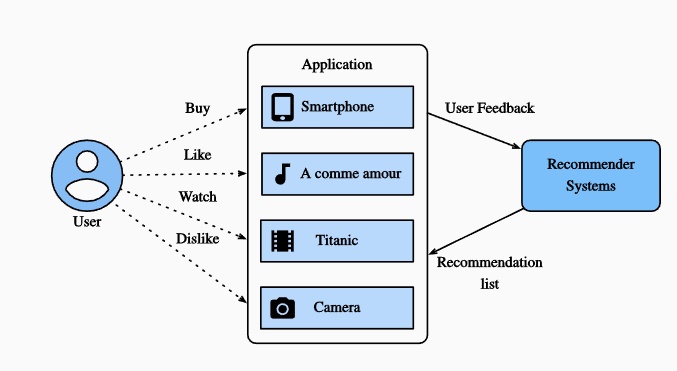
\includegraphics[width=0.7\linewidth]{Figures/RS.png}
	\caption{Recommendation System Process}
	\label{Recommendation_System _Process}	
	\end{figure}

\subsection{Types of Recommendation Systems}

Recommendation systems can be broadly categorized into several types based on their underlying methodologies~\citep{maruti_recsys}:

\begin{enumerate}
	\item \textbf{Content-Based Filtering:} This approach recommends items similar to those the user has liked in the past, based on item features. It relies on the assumption that if a user liked an item, they will also like similar items.
	
	\item \textbf{Collaborative Filtering:} This method predicts user preferences based on the preferences of other users. It operates under the premise that users who agreed in the past will agree in the future about item preferences.
	
	\item \textbf{Hybrid Methods:} These systems  integrate both content-based and collaborative filtering approaches to enhance the accuracy and diversity of suggestions. A well-known example is Netflix, which combines user behavior patterns (e.g., viewing and search history) with similarities across users to implement collaborative filtering, while also recommending content with attributes similar to previously liked items via content-based filtering.
	
	\item \textbf{Sequential Recommendation Models:} These models consider the sequence of user interactions over time to predict future preferences. An example is the Self-Attentive Sequential Recommendation \textbf{(SASRec)} model, which utilizes self-attention mechanisms to capture user behavior patterns effectively. SASRec has demonstrated superior performance in modeling user-item interactions by focusing on the most relevant past actions.
\end{enumerate}

\subsection{Evaluation Metrics}

Evaluating the performance of recommendation systems is crucial for understanding their effectiveness and guiding improvements. Common evaluation metrics include:

\begin{itemize}
	\item \textbf{Hit Rate at \( k \) (HR@\( k \))}: Measures the proportion of cases where the target item appears in the top-\( k \) recommendations. The HR@\( k \) is computed as:\citep{Tamm_2021}
	\begin{equation}
		\text{HR@}k = \frac{1}{|U|} \sum_{u=1}^{|U|} \mathbb{I}(\text{rank}_u \leq k),
	\end{equation}
	where \( |U| \) is the number of users, \( \text{rank}_u \) is the rank of the target item for user \( u \), and \( \mathbb{I}(\cdot) \) is the indicator function that returns 1 if the condition is true and 0 otherwise.
	
	\item \textbf{Mean Reciprocal Rank (MRR)}:is a ranking quality metric that measures how quickly a system retrieves the first relevant item. It is calculated as the average of reciprocal ranks across all users or queries,MRR ranges from 0 to 1, with higher values indicating better performance \citep{Tamm_2021}.
	\begin{equation}
		\text{MRR} = \frac{1}{|U|} \sum_{u=1}^{|U|} \frac{1}{\text{rank}_u},
	\end{equation}
	where \( \text{rank}_u \) is the position of the first relevant item for user \( u \) within the top-K results. \\ 
	U represents the total number of users (for recommendation systems) or queries (for information retrieval tasks) in the dataset.
	
	\item \textbf{Normalized Discounted Cumulative Gain (NDCG)}: Assesses the ranking quality while accounting for position importance. The NDCG@\( k \) is computed as:\citep{Tamm_2021}
	\begin{equation}
		\text{NDCG@}k = \frac{1}{|U|} \sum_{u=1}^{|U|} \frac{\text{DCG@}k}{\text{IDCG@}k},
	\end{equation}
	where \( \text{DCG@}k \) is the Discounted Cumulative Gain at position \( k \):
	\begin{equation}
		\text{DCG@}k = \sum_{i=1}^{k} \frac{2^{\text{rel}_i} - 1}{\log_2(i + 1)},
	\end{equation}
	and \( \text{IDCG@}k \) is the Ideal DCG@\( k \), computed by sorting the items by their true relevance scores.
\end{itemize} 

\subsection{Retrieval-Augmented Generation in Recommendation Systems}

Retrieval-Augmented Generation represents a significant advancement in recommender systems by integrating large language models LLMs with traditional retrieval techniques. This approach enhances recommendation quality by allowing the system to access and incorporate external information into its responses, resulting in more accurate and context-aware suggestions.

In this setup, a RAG-based recommender retrieves relevant data from external sources and feeds it into the language model, which then generates personalized recommendations based on both the retrieved content and user input\citep{DiPalma}. This hybrid mechanism helps overcome common challenges like the cold start problem and data sparsity, enabling effective recommendations even with limited user history.

Recent studies highlight that combining retrieval with LLMs greatly improves the system’s ability to deliver more relevant and diverse content, offering a promising direction for improving user experience in applications such as e-commerce and digital streaming platforms.



\section{Conclusion}


In this chapter, we explored the core principles and mechanisms of RAG, emphasizing its potential to enhance language models through access to external knowledge sources during inference. We examined its general architecture, key stages, and its evolution from naive to more modular frameworks. 

Particular attention was given to RAG’s application in the legal domain, highlighting its ability to enhance legal information retrieval by enabling more contextualized and semantically rich access to case law, statutes, and scholarly texts. We also outlined the main challenges and limitations facing RAG models. Additionally, the chapter briefly touched on the integration of RAG in recommendation systems, introducing its potential to improve personalization and relevance in such applications.

the next chapter addresses a critical factor in RAG performance: knowledge selection. Specifically, we explore how the effectiveness of retrieved documents directly influences the quality of generated responses, and we investigate strategies to improve relevance and ranking within RAG pipelines.
 
		\chapter{k-Selection Optimization in RAG }
\pagestyle{fancy}\lhead{\textbf \footnotesize\it{k-Selection Optimization in RAG }}
\pagestyle{fancy}\chead{} \pagestyle{fancy}\rhead{} 
\pagestyle{fancy}\cfoot{} \pagestyle{fancy}\rfoot{\thepage}
%%%%%%%%%%%%%%%%%%%%%%%%%%%%%%%%%%%%%%%%
\section{Introduction}
Retrieval-Augmented Generation systems enhance language models by grounding responses in externally retrieved documents. A critical challenge is determining the optimal number of documents k to retrieve for a given query. In this chapter, we first explore methods, highlighting their strengths and limitations We then introduce our novel hybrid dynamic selection algorithm provide detailed description of its methodology and present experimental results that demonstrate the effectiveness of its performance . 

\section{Defining k: The Number of Retrieved Documents}
the parameter k denotes the number of documents or passages retrieved from an external knowledge base. This retrieval process is managed by the retriever component\citep{pareto2024rag},which identifies the top k relevant documents based on similarity to the query typically using embedding-based search\citep{Rossi_2024} (e.g., dense retrieval with FAISS, BM25, or hybrid methods) Subsequently, these documents are passed to the generator, typically a language model, which synthesizes the final response by integrating the retrieved 
\begin{figure}[h]
	\centering
	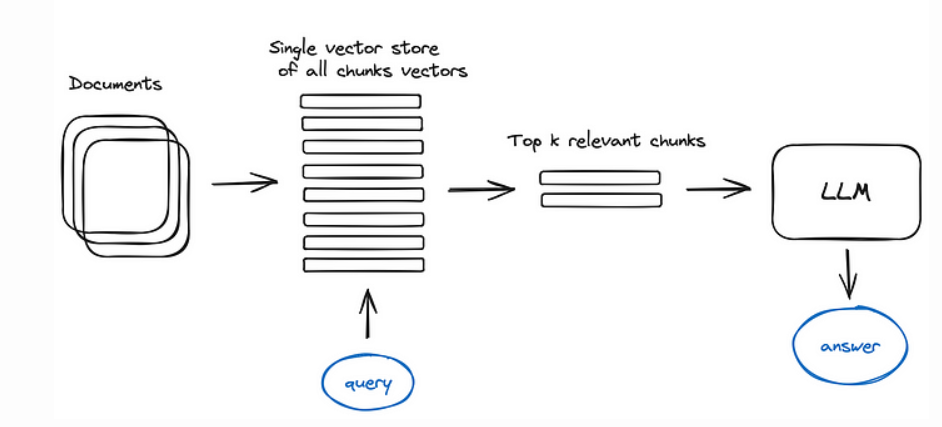
\includegraphics[width=0.9\linewidth]{Figures/topk.png}
	\caption{Basic retrieval}
	\label{rag_retrival.png}
	
\end{figure}

\section{Impact of k on Retrieval Performance}
The retriever's effectiveness in identifying relevant documents depends on k. Key impacts include :
\subsection{Recall vs. Precision} 
When a user conducts a search query, the outcomes from the database can be grouped into four distinct types based on relevance and retrieval status \citep{geeksforgeeks2022precision}:
\begin{itemize}
	\item {Relevant and Retrieved:} Documents that both address the user’s query and appear in the search results.
	\item {Relevant and Not Retrieved:} Useful documents that answer the query but are not included in the results.
	
	\item {Non-Relevant and Retrieved:} Documents that appear in the results but lack meaningful value for the query.
	 
	\item {Non-Relevant and Not Retrieved:} Irrelevant documents excluded from the results.
\end{itemize}


\textbf{Precision@k}: evaluates the proportion of relevant documents within the top k retrieved results. This metric is particularly valuable in scenarios where the focus is on delivering highly relevant information quickly, rather than ensuring complete coverage such as ,recommendation systems or search engines\citep{deconvoluteai2024metrics}.
\begin{equation}
\text{Precision@k} = \frac{\text{Number of Relevant Items Retrieved in Top k}}{k}
\end{equation}
\textbf{Example}
Suppose we have a dataset of 10 documents. If we retrieve \( k = 4 \) documents and find that 3 of them are relevant to the query:

\begin{itemize}
	\item \textbf{Dataset}: [doc1, doc2, doc3, doc4, doc5, doc6, doc7, doc8, doc9, doc10]
	\item \textbf{Retrieved}: [doc3, doc1, doc7, doc4]
	\item \textbf{Relevant}: [doc1, doc3, doc5, doc8]
\end{itemize}

The Precision@4 score would be:

\begin{equation}
\text{Precision@4} = \frac{3}{4} = 0.75
\end{equation}


\textbf{Recall@k :}Evaluates the proportion of relevant documents that are successfully retrieved within the top k results. This metric is particularly important in contexts where ensuring the completeness of information is crucial, such as in medical research or academic tools, where omitting relevant documents could result in incomplete or inaccurate conclusions\citep{deconvoluteai2024metrics}.
\begin{equation}
\text{Recall@k} = \frac{\text{Number of Relevant Items Retrieved in Top k}}{\text{Total Number of Relevant Items}}	
\end{equation}
\textbf{Example:}
Consider a dataset of 10 documents. If we retrieve \( k = 4 \) documents and find that 2 of them are relevant, while the total number of relevant documents in the dataset is 4
\begin{equation}
\text{Recall@4} = \frac{2}{4} = 0.5
\end{equation}
Increasing k typically enhances recall by retrieving more relevant documents but may decrease precision due to the inclusion of irrelevant ones. Conversely, decreasing k can improve precision but at the cost of lower recall. 
\subsection{Retrieval Speed and Computational Cost}
Retrieval speed and computational cost are two important areas where k has a big influence Below is a detailed explanation of how higher k values affect these aspects.

\textbf{Increased Computational Resources:} \\
As the value of k expands, the retrieval must handle a larger set of documents, leading to higher computational demands. Specifically, the system needs to perform additional operations like ranking, filtering, and similarity scoring to identify the most relevant documents. These tasks become increasingly resource-intensive, particularly in large-scale retrieval settings where the document corpus consists of millions or even billions of entries\citep{manning2008ir}. For instance, retrieving the top  documents (k=80) requires significantly more computational resources compared to retrieving only the top 10 documents (k=5). 

\textbf{Higher Memory Usage:}
As the number of retrieved documents k increases, Storing and processing a larger set of retrieved documents requires more memory This can become a significant bottleneck, especially in environments with constrained memory resources.

For large-scale retrieval tasks, where datasets may contain millions or even billions of documents, the memory demand grows proportionally with k. Each retrieved document needs to be stored temporarily, along with its associated metadata, such as embedding vectors, BM25 scores, or other relevance signals. Additionally, sorting and filtering operations further contribute to memory overhead
\subsection{Document Ranking Quality}
Document ranking in information retrieval involves ordering documents by their relevance to a user's query. The objective is to prioritize the most relevant documents at the top of search results, making it easier for users to access useful information quickly. Different models,Vector Space, including Boolean, and Probabilistic models, are used to establish this ranking \citep{enwiki:1262179867}.\\

Increasing the number of retrieved documents,represented as k, may result in the addition of lower-ranked, less relevant documents, potentially diluting the overall quality of the retrieved information. This occurs because of the inherent balance between precision and recall in information retrieval systems.
\begin{figure}[h]
	\centering
	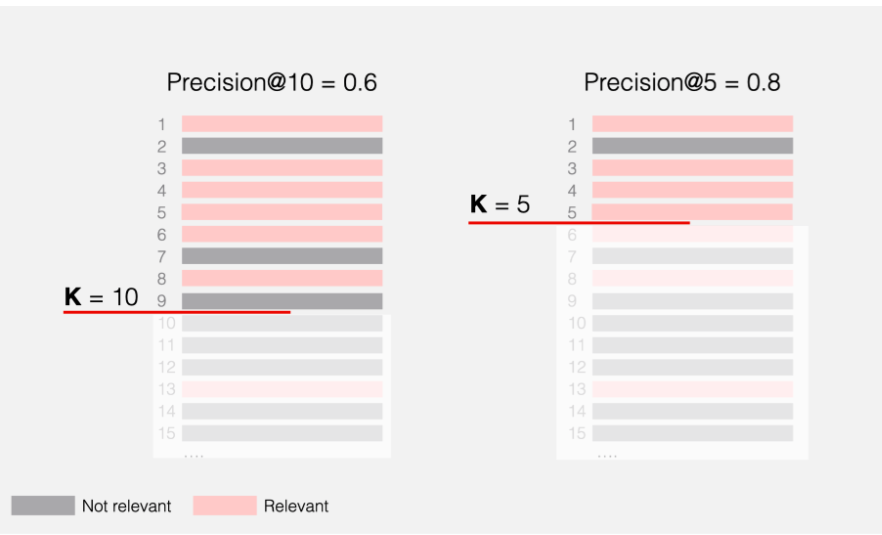
\includegraphics[width=0.7\linewidth]{Figures/precisionR.png}
	\caption{Precision in Document Ranking}
	\label{precisionR}
	
\end{figure}

\begin{figure}[h]
	\centering
	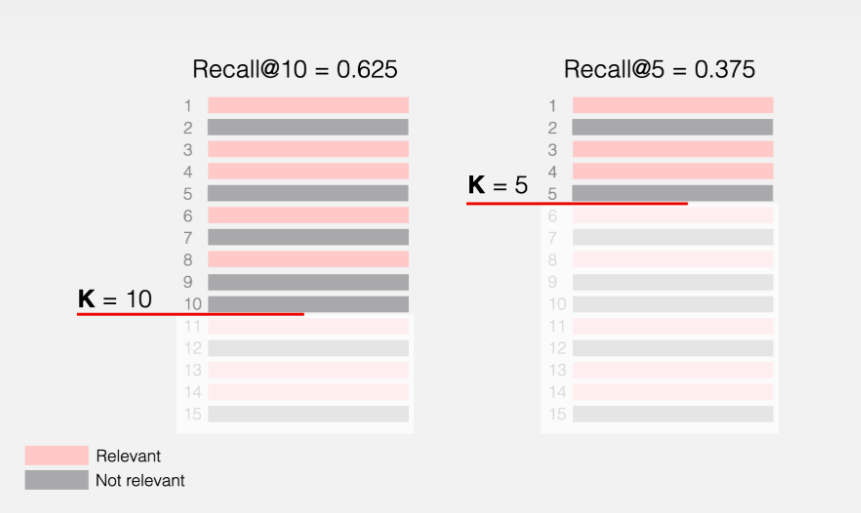
\includegraphics[width=0.7\linewidth]{Figures/recalR.png}
	\caption{Recall in Document Ranking}
	\label{recalR}
	
\end{figure}
As k grows, recall generally improves since a larger number of relevant documents are likely to be retrieved as shown in Figure \ref{recalR}. However, this often comes at the expense of precision, as the additional documents retrieved may include non-relevant ones, thereby lowering the overall precision as illustrated in Figure \ref{precisionR}. This trade-off is a core principle in evaluating information retrieval systems.

\section{Impact of k on Generation Quality}
The impact of k (the number of retrieved documents or generated candidates) on generation quality is A crucial factor in many machine learning and information retrieval tasks, including text generation, recommendation systems, and search engines. 

\subsection{Trade-off Between Diversity and Relevance} 
\textbf{Higher k:} Increasing k often improves diversity in generated outputs or retrieved documents, as more candidates are considered. However, this can lead to a drop in relevance or quality, as lower-ranked candidates may be less accurate or coherent. \\
\textbf{Lower k:} A smaller k tends to prioritize high-quality, relevant outputs but may lack diversity, leading to repetitive or overly narrow results.

Research shows that the quality of retrieved documents plays a crucial role in the performance of RAG . For example, one study demonstrated that the precision of retrieved documents directly affects the factual correctness of the generated responses \citep{salemi2023evaluating}
Additionally, another study \citep{wan2025cognitivealigneddocumentselectionretrievalaugmented} revealed that simply increasing the number of documents does not necessarily improve generation quality, especially if the additional documents are not highly relevant.
\subsection {Effect on Text Generation Models}
In text generation tasks, such as machine translation and dialogue systems, The parameter k frequently refers to the beam width in beam search algorithms\citep{freitag-al-onaizan-2017-beam}.Beam search is a heuristic search algorithm that expands the most promising nodes in a graph to maximize the quality of the text that is produced. Adjusting the beam width k has significantly impacts how well text generation models function.

As the beam width is increased, the model must process and retain more candidate sequences concurrently, leading to higher computational and memory demands Particularly in real-time applications where latency is crucial\citep{tensorrt_llm_beam_search}, this increase may have an effect on system performance and response time.

\section{Existing Solutions for k Selection}
Selecting an optimal k plays a crucial role in balancing retrieval effectiveness and generation quality. Over the years, various strategies have been proposed to determine k, ranging from static selection to dynamic and hybrid approaches.
\subsection{Static k Selection}
In RAG, "static k selection", refers to the process of setting a fixed number of top documents k to retrieve for every query, irrespective of how simple or complex the query might be. This approach simplifies the retrieval process by maintaining a consistent retrieval count across all queries.

\subsubsection{Sparse Retrieval with Fixed k} 
Sparse retrieval is a method of finding relevant documents from a large collection by representing both queries and documents as vectors where most values are zero\citep{zheng2024enhancing}. This focus on only the most important terms leads to faster, more accurate searches, especially useful when combining information from different sources 
Common approaches include. \textbf{BM25}\citep{10.1561/1500000019} where documents are scored for relevance by considering term frequency and inverse document frequency, it selects the k documents with the highest BM25 scores for each query,\textbf{TF-IDF} (Term Frequency-Inverse Document Frequency)\citep{gfg2025tfidf}in this method the retrieved documents would be those with the highest weighted term importance, Other methods like \textbf{QLM }(Query Likelihood Model)\citep{10.1007/978-3-030-72240-1_49}use probabilistic models to evaluate the likelihood of a query and rank documents according to textual similarity.

\subsubsection{Dense Retrieval with Fixed k} 
Dense retrieval \citep{karpukhin2020dense} is a method for retrieving information that uses deep learning models to convert documents and queries into high-dimensional vector embeddings, a fixed number of top-k documents are selected based on similarity scores between the query embedding and document embeddings in a continuous vector space, the retrieval process allows the system to capture semantic elationships beyond exact term matches.

Methods such as dual-encoder architectures (e.g., DPR - Dense Passage Retrieval)\citep{chen-etal-2024-dense} utilize separate neural networks (encoders) for queries and documents enable efficient retrieval, while Approximate Nearest Neighbor (ANN) search techniques (e.g., FAISS)\citep{enwiki:1276232158} optimize search efficiency in large-scale datasets .
\subsection{Dynamic k Selection}
In retrieval, dynamic k selection is the process of varying the quantity of documents k that are retrieved according to the properties of the query, such as its ambiguity, complexity, or relevance score distribution. This approach is crucial for enhancing the effectiveness and efficiency of information retrieval systems.

\subsubsection{Dynamic Trade-Off Prediction in Multi-Stage Retrieval Systems } This approach predicts the optimal number of documents k to retrieve. It uses pre-retrieval features to balance the trade-off between retrieval efficiency and effectiveness, ensuring that the system retrieves an appropriate number of documents for each query\citep{culpepper2016dynamictradeoffpredictionmultistage}.

\subsubsection{Dynamic Pruning Methods:}
This approach addresses the challenge of balancing effectiveness and efficiency in large-scale Information Retrieval systems, particularly under temporal constraints. The goal is to process queries within a specified time limit while minimizing the loss in retrieval effectiveness.\citep{10.1007/978-3-319-70145-5_1} The authors propose and evaluate three techniques for temporally constrained top-K query processing .
\subsection{Hybrid k Selection}
hybrid methods aim to achieve optimal retrieval By merging static and dynamic k selection, These methods balance computational efficiency (from static k) with adaptive flexibility (from dynamic k) ensuring high-quality retrieval Below are some key hybrid strategies.

\subsubsection{Blended RAG} 
An innovative method to improve Retrieval-Augmented Generation systems, which integrate private document collections with Large Language Models for Generative Question-Answering it employs a hybrid retrieval approach, combining Dense Vector indexes and Sparse Encoder indexes with sophisticated query strategies\citep{sawarkar2024blendedragimprovingrag}., Blended RAG provides a scalable and efficient solution for enhancing RAG, showcasing the effectiveness of merging dense and sparse retrieval techniques.

\subsubsection{ STAYKATE (Static-Dynamic Hybrid Selection)}
A new approach for selecting in-context examples to improve the performance of LLMs in scientific information extraction. Scientific tasks often struggle with limited training data and expensive annotation processes. STAYKATE tackles these challenges by merging static and dynamic selection strategies \citep{zhu2024staykatehybridincontextexample}, combining representativeness sampling from active learning with retrieval-based methods. This hybrid approach ensures the selection of high-quality, informative examples, enhancing in-context learning for LLMs.
\section{Proposed Solution}
While existing k-selection approaches—static, dynamic, and hybrid—offer distinct advantages, they also present notable limitations, such as lack of adaptability in static k selection, which fails to adjust for query complexity, leading to either missing relevant documents or retrieving irrelevant ones. Dynamic k selection, while more flexible, introduces higher computational costs and requires carefully tuned heuristics, making it challenging to scale. Hybrid approaches, attempt to balance both strategies but suffer from increased system complexity.

To address these challenges, we propose an enhanced k-selection strategy that optimally balances retrieval efficiency and relevance, leveraging adaptive mechanisms to improve performance across diverse query types. Table \ref{tab:Notations_table} summarizes the notations used in this work.

\begin{table}[h]
	\centering
	 % Increase overall font size
	\begin{tabular}{|c|p{13cm}|}  % Use p{width} for text wrapping
		\hline
		\textbf{Notation} & \textbf{Description} \\ \hline
		\( q \) (\( Q \), \( |Q| \)) & A single query (set of all queries, total number of queries). \\ \hline
		\( x \) (\( X \), \( |X| \)) & A single item (set of all items, total number of items). \\ \hline
		\( \phi(q, x) \) & The learned similarity function, Mixture-of-Logits (MoL), which computes the similarity between \( q \) and \( x \). \\ \hline
		\( P \) (\( P_q \), \( P_x \)) & Total number of low-rank embeddings (\( P = P_q \times P_x \)), where \( P_q \) and \( P_x \) are the number of embeddings for \( q \) and \( x \), respectively. \\ \hline
		\( \pi_p(q, x) \)  & Weight for the \( p \)-th (or \( p_q \)-th and \( p_x \)-th) embedding set for \( (q, x) \). \\ \hline
		\( f(q) \) (\( f_p(q) \)) & Learned embedding for the query (\( p \)-th component-level embedding for \( q \)). \\ \hline
		\( g(x) \) (\( g_p(x) \)) & Learned embedding for the item (\( p \)-th component-level embedding for \( x \)). \\ \hline
		\( \langle f(q), g(x) \rangle \) & Dot product similarity function: \( \langle f(q), g(x) \rangle = g(x)^T f(q) \). \\ \hline
	\end{tabular}
	\caption{Notation Table }
	\label{tab:Notations_table}
\end{table}

\newpage
\subsection{Mixture of Logits (MoL)}

The \textbf{Mixture of Logits (MoL)}\citep{zhai2023revisiting,Ding2024}  approach is designed to enhance retrieval and ranking by leveraging multiple low-rank embeddings. It assumes that both the \textbf{query} (\( q \)) and \textbf{document/item} (\( x \)) are mapped into \( P \) groups of low-dimensional embeddings, denoted as \( f_p(q) \) and \( g_p(x) \), which are generated by neural networks based on their respective features.
\begin{figure}[h]
	\centering
	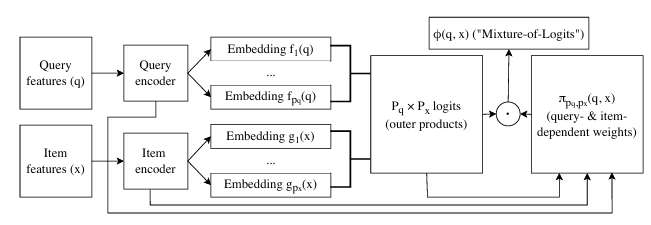
\includegraphics[width=0.7\linewidth]{Figures/mol.png}
	\caption{Mixture of Logits(MoL) learned similarity.}
	\label{Mixture_of_Logits }	
\end{figure}
To determine the similarity between a query and a document, MoL assigns \textbf{adaptive gating weights} \( \pi_p(q,x) \) to the inner products of these low-rank embeddings\citep{zhai2023revisiting}:

\begin{equation}
	\phi(q,x) = \sum_{p=1}^{P} \pi_p(q,x) \langle f_p(q), g_p(x) \rangle
\end{equation}

where \( \pi_p(q,x) \) represents the learned weights for each component, ensuring that their sum equals one. These weights are typically parameterized using a neural network that takes embeddings and their inner products as input features.

To efficiently scale MoL for large datasets and hardware-optimized implementations, the formulation is extended by decomposing the dot products into \textbf{batched outer products} of query-side and document-side embeddings. This decomposition improves computational efficiency, particularly on accelerators like GPUs, by normalizing the embeddings using the \( l_2 \)-norm:\citep{zhai2023revisiting}

\begin{equation}
	\phi(q,x) = \sum_{pq=1}^{P_q} \sum_{px=1}^{P_x} \pi_{pq,px}(q,x) \frac{\langle f_{pq}(q), g_{px}(x) \rangle}{|| f_{pq}(q) ||_2 || g_{px}(x) ||_2}
\end{equation}

Since embedding normalization can be precomputed, both formulations remain interchangeable in practical applications. Furthermore, it is possible to \textbf{decompose any high-rank matrix} into a mixture of logits based on low-rank matrices, demonstrating the flexibility and scalability of this approach in large-scale information retrieval tasks.
\subsection{Algorithm Design}
we introduce an adaptive threshold mechanism
(Dynamic K-Selection for Optimal Retrieval), the MoL framework is employed to refine the
candidate retrieval process. 
\begin{figure}[ht]
	\centering
	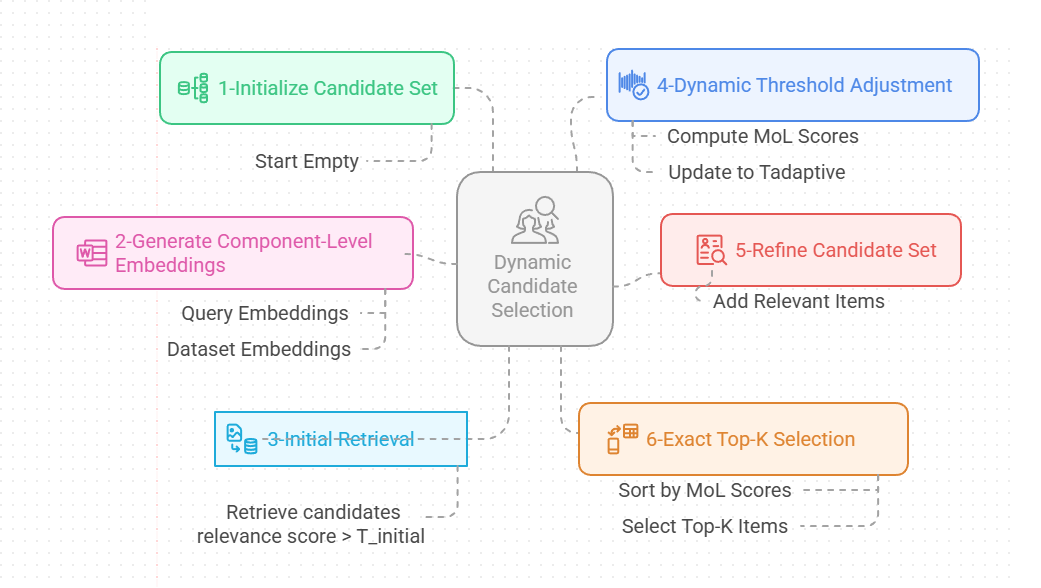
\includegraphics[width=0.7\linewidth]{Figures/propused _solution_steps.png}
	\caption{propused solution steps}
	\label{propused _solution_steps}	
\end{figure}

\noindent

1. \textbf{Component-Level Embeddings}:  
Component-level embeddings are generated for all items in the dataset \(X\). These embeddings facilitate efficient similarity computations during retrieval. Formally,
\begin{equation}
	X_p \leftarrow \{g_p(x) \mid x \in X\}.
\end{equation}

\noindent
2.\textbf{ Initial Candidate Retrieval:} This step involves computing similarity scores between a query representation and item representations for each feature component $p \in P$.  

\begin{equation}
	S_p \gets  \{ \langle f_p(q), g_p(x) \rangle : x \in X_p \}
	\label{eq:initial_retrieval}
\end{equation}
Here, $f_p(q)$ and $g_p(x)$ represent the feature embeddings of the query $q$ and item $x$ for the $p$-th component, respectively. The dot product $\langle f_p(q), g_p(x) \rangle$ measures the relevance of each item $x \in X_p$ with respect to $q$, producing a set of scores $S_p$ .


\noindent
3. \textbf{Dynamic Threshold Adjustment}:  
To improve retrieval quality, \textbf{Mixture of Logits (MoL)} scores are computed for each candidate \(x \in G\). The adaptive gating weights \(\pi_p(q, x)\) allow the algorithm to dynamically adjust the retrieval threshold \(T_{\text{adaptive}}\) based on the MoL scores. The scoring function is defined as:
\begin{equation}
	\phi(q, x) = \sum_{p=1}^{P} \pi_p(q, x) \cdot \langle f_p(q), g_p(x) \rangle.
	\label{similarity_function}
\end{equation}
The adaptive threshold \(T_{\text{adaptive}}\) is set as the minimum score among the candidates:
\begin{equation}
	T_{\text{adaptive}} = \min\{s \mid s \in G\}.
\end{equation}

\noindent
4. \textbf{Refinement and Top-K Selection}:  
Using the adaptive threshold \(T_{\text{adaptive}}\), additional relevant candidates are retrieved, expanding the candidate set \(G'\). This is achieved by including candidates whose scores exceed the threshold:
\begin{equation}
	G' \leftarrow G \cup \{x \mid s_p \geq T_{\text{adaptive}}\}.
\end{equation}
The algorithm then sorts \(G'\) based on MoL scores to select the most relevant top-k candidates.

\noindent
4. \textbf{Exact Top-K Selection}:  
Finally, the candidates in \(G'\) are sorted by their MoL scores, and the exact top-k items are extracted:
\begin{equation}
	G_{\text{final}} = \text{Top-k}(G', \phi(q, x)).
\end{equation}
As shown in Algorithm\ref{ALgo1}, the retrieval process dynamically adjusts the threshold based on MoL scores.



\subsection{Hybrid k-Selection Algorithm Pseudocode}
The following pseudocodeAs shown in Algorithm\ref{ALgo1} outlines our proposed Dynamic K-Selection for Optimal Retrieval algorithm. This method adaptively selects the number of top-k documents retrieved based on query characteristics, enhancing the relevance and efficiency of the retrieval step in our RAG pipeline

\begin{algorithm}
	\caption{Hybrid Exact Top-k with Threshold-Based k Selection}
	\label{ALgo1}
	\textbf{Input:} Query $q$, Set of items $X$, Component-level embeddings: $f_p(q)$, $g_p(x)$ for $p \in P$, $x \in X$, Initial threshold $T_{\text{init}}$ \\
	\textbf{Output:} Exact top $k$ items based on dynamic threshold   selection, $G_{\text{final}}$
	
	\begin{algorithmic}[1]
		
		
		\State Set $G \gets \emptyset$     \Comment{Initial candidate set}
		\For{each component $p \in P$}
		\State $X_p \gets \{g_p(x) \mid x \in X\}$ \Comment{Precompute embeddings}
		\EndFor
		
		\textbf{1. Initial Candidate Retrieval:}
		\For{each component $p \in P$}
		\State Compute dot product scores:  with (eq\eqref{eq:initial_retrieval})
		
		\State Retrieve items with scores $S_p \geq T_{\text{init}}$
		\State Add these items to $G$
		\EndFor
		
		\textbf{2. Adjust k Dynamically:}
		\For{each $x \in G$}
		\State Compute MoL scores $s \gets \phi(q, x)$ using : eq\eqref{similarity_function}
		\State Set $T_{\text{adaptive}} = \min \{s : s \in G\}$
		\EndFor
		
		\textbf{3. Refine Candidate Set with Adaptive k:}
		\State	$G' \gets \emptyset$
		\For{each component $p \in P$}
		\State Retrieve items from $X_p$ with scores $S_p \geq T_{\text{adaptive}}$
		\State Add these items to $G'$
		\EndFor
		
		\textbf{4. Select Exact Top-k Items:}
		\For{each component $p \in P$}
		\State Compute MoL scores for all items in $G'$
		\State Sort $G'$ by MoL scores in descending order
		\State Select the top $k$ items from $G'$ where $k$ is the number of items in $G'$ exceeding $T_{\text{adaptive}}$
		\EndFor
		\State\textbf{ Return:} $G_{\text{final}}$ \Comment{Retrieve Top $k$ items from $G'$}
	\end{algorithmic}
\end{algorithm}

\newpage

\section{Experimental Results}\label{sec3}
In order to measure the effectiveness of our proposed method, we perform a comprehensive evaluation of both the retrieval algorithm and the Mixture-of-Logits (MoL) approach. This assessment focuses on the next-item prediction task, a fundamental challenge in recommendation systems\citep{kang2018selfat},
where the goal is to predict the most relevant item a user will interact with next based on their past interactions. 
\subsection{Dataset Design}
We conducted experiments using two MovieLens datasets : ML-100K and ML-1M \citep{Harper2015}which are widely used benchmarks for evaluating sequential recommendation models as detailed in Table\ref{tab_movielens}.\\
\begin{table}[h]
	\centering
	\renewcommand{\arraystretch}{1.2}
	\begin{tabular}{|l|p{10cm}|}
		\hline
		\textbf{Dataset} & \textbf{Description} \\
		\hline
		\textbf{MovieLens-100K} & 100,000 ratings (1-5 scale) from 943 users on 1,682 movies. \\
		& Each user has rated at least 20 movies. \\
		& Includes user demographic information (age, gender, occupation, zip code). \\
		\hline
		\textbf{MovieLens-1M} & 1,000,209 ratings from 6,040 users on approximately 3,900 movies. \\
		& Data collected from users who joined MovieLens in 2000. \\
		& Represents a larger-scale recommendation scenario. \\
		\hline
	\end{tabular}
	\caption{Summary of MovieLens datasets}
	\label{tab_movielens}
\end{table}

\subsection{Experimental Setup }
For both datasets, We utilize the SASRec architecture as our sequential user encoder, a model renowned for achieving state-of-the-art performance in next-item prediction tasks. This architecture processes the user's historical interaction sequence, generating embeddings that encapsulate the user's preferences at each time step. These embeddings serve as the foundation for predicting the next item in the sequence.

The query \( q \) represents the user's state at a specific time step, derived from their interaction history. In the MoL (Mixture of Logits) framework,\( q \)is transformed into \( Pq \)
embeddings through a multi-layer perceptron (MLP).

For fair comparison, we maintained consistent architectural choices and training conditions across all experiments, We conducted an extensive hyperparameter analysis comparing both approaches (Hybrid+SAS and MoL+SAS) across different architectural configurations:
\subsubsection{Fixed Experimental Configuration}
\begin{itemize}
	\item \textbf{Hardware}: Google Colab with T4 GPU
	\item \textbf{Framework}: TensorFlow
	\item \textbf{Optimizer}: Adam ($\eta=0.001$)
	\item \textbf{Hybrid Specific}: $T_{init}=0.3$ (init threshold)
     
\end{itemize}
For the hybrid algorithm, we initialize the threshold (Tinit) to 0.3 and adaptively adjust it during training. We discuss detailed hyperparameter settings in table \ref{tab:all_results}, table
\subsection{Architectural Variants and Results}

The following tables present our complete experimental results across different model configurations. 
\begin{table}[h]
	\centering
	
	\resizebox{\textwidth}{!}{
		\begin{tabular}{lccccccc}
			\toprule
			\multirow{2}{*}{\textbf{Model}} & 
			\multirow{2}{*}{\textbf{SeqLen}} & 
			\multirow{2}{*}{\textbf{EmbDim}} & 
			\multirow{2}{*}{\textbf{Heads}} & 
			\multicolumn{2}{c}{\textbf{100kMovies}} & 
			\multicolumn{2}{c}{\textbf{1M Movies}} \\
			\cmidrule(lr){5-6} \cmidrule(lr){7-8}
			& & & & Val Loss & Val Acc & Val Loss & Val Acc \\
			\midrule
			Hybrid+SAS & 50 & 128 & 2 & 5.3036 & 0.1584 & 4.5721 & 0.1530 \\
			MoL+SAS & 50 & 128 & 2 & 5.3152 & 0.1582 & 4.5733 & 0.1526 \\
			\addlinespace
			Hybrid+SAS & 128 & 256 & 4 & 3.6364 & 0.4301 & 3.4152 & 0.3680 \\
			MoL+SAS & 128 & 256 & 4 & 3.6374 & 0.4299 & 3.4671 & 0.3627 \\
			\addlinespace
			Hybrid+SAS & 512 & 512 & 4 & 1.2808 & \textbf{0.8120} & 1.0275 & \textbf{0.8350} \\
			MoL+SAS & 512 & 512 & 4 & 1.3050 &\textbf{ 0.8016} & 1.0350 &\textbf{ 0.8276 }\\
			\bottomrule
		\end{tabular}
		
	}
	\caption{Performance Across Configurations}
	\label{tab:all_results}
\end{table}

Both approaches demonstrate significant performance improvements as model capacity increases, with larger configurations consistently delivering better results. For instance, when increasing the model's capacity such as expanding the (Max Sequence Length: 512, Embedding Dimension: 512, Number of Heads: 4, Feed-Forward Dimension: 512) the hybrid algorithm combined with SASRec (Hybrid+SAS) achieves notable gains, particularly in the most resource-intensive setup. On the ML-100K dataset, Hybrid+SAS reaches a score of\textbf{0.8120} compared to the baseline's \textbf{0.8016}, while on ML-1M, it achieves \textbf{0.8350} versus \textbf{0.8276} The ML-1M dataset generally benefits more from increased capacity, with the performance gap between datasets narrowing as the model scales. While smaller configurations provide a balance of efficiency and performance, the largest configuration, despite its higher computational demands, yields the best results, making it suitable for scenarios where resources are not a constraint. Both approaches show similar benefits from scaling, but Hybrid+SAS maintains a consistent edge in performance.


\subsection {Impact of Adaptive k-Variations on Model Performance}
As shown in Figures~\ref{fig:k_changes_100K} and \ref{fig:k_changes_1M}, the value of $k$ fluctuates across epochs for both MovieLens 100K and MovieLens 1M datasets. These variations indicate the adaptive nature of $k$ in response to the dataset characteristics and training progress. In the following section, we analyze how these changes influence model performance.  

\begin{figure}[htbp]
	\centering
	\begin{subfigure}{0.48\textwidth}
		\centering
		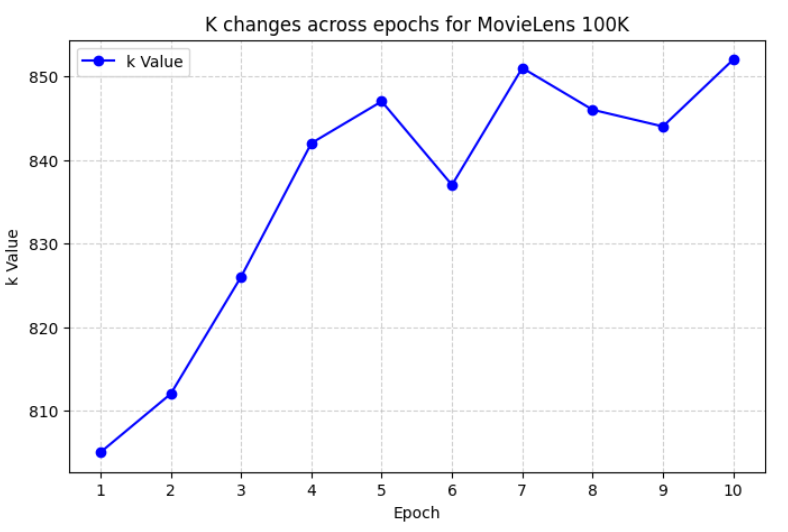
\includegraphics[width=\linewidth]{Figures/CHAGES_OF_K_FOR_100k.png}
		\caption{K changes across epochs for MovieLens 100K}
		\label{fig:k_changes_100K}
	\end{subfigure}
	\hfill
	\begin{subfigure}{0.48\textwidth}
		\centering
		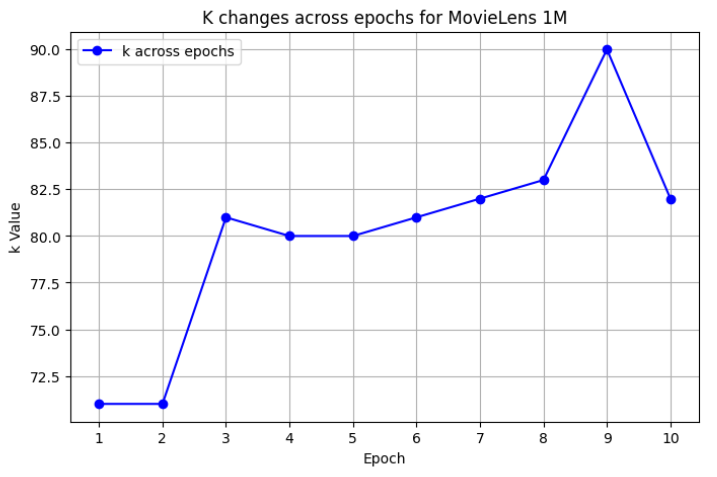
\includegraphics[width=\linewidth]{Figures/chnages_inK_for_1M.png}
		\caption{K changes across epochs for MovieLens 1M}
		\label{fig:k_changes_1M}
	\end{subfigure}
	\caption{Comparison of K changes across epochs for different datasets}
	\label{fig:k_changes}
\end{figure}
the value of K changed dynamically during training, with different behaviors. For the MovieLens 100K dataset, K showed a steady increase across epochs, whereas for the MovieLens 1M dataset, K began at a lower value, experienced fluctuations, peaked, and then stabilized. This indicates that the larger dataset necessitated more adaptive adjustments in retrieval compared to the smaller dataset.\\
Figure~\ref{histo_p} summarizes the performance of our hybrid algorithm compared to the MoL-based approach on the MovieLens 100K and 1M datasets, both tested using a Max Sequence Length of 50, an Embedding Dimension of 128, 2 Attention Heads, a Feedforward Dimension of 128, a Batch Size of 128, and trained for 10 epochs . \\
\begin{figure}[ht]
	\centering
	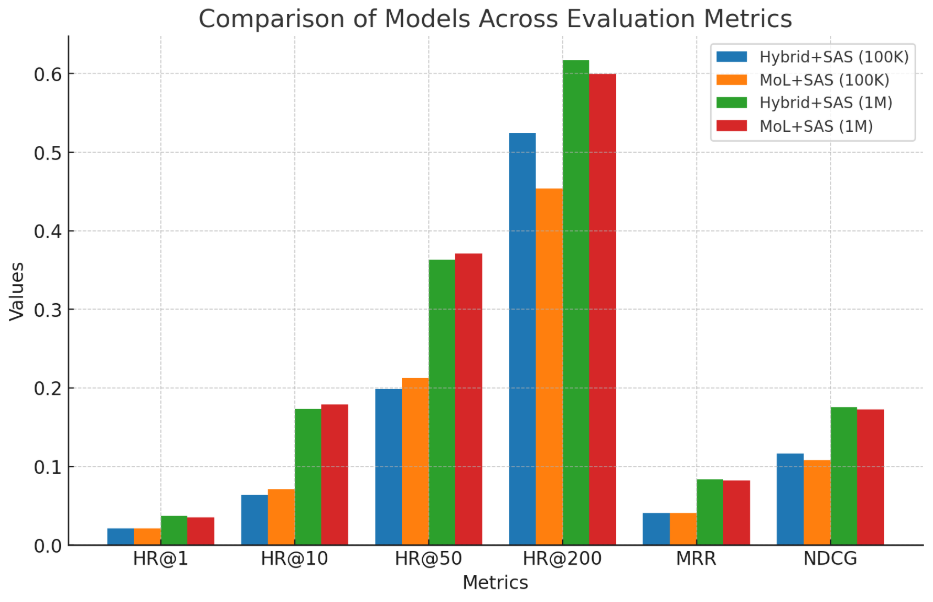
\includegraphics[width=0.7\textwidth]{Figures/HISTOGRAM.png}
	\caption{Comparison of Models Across Evaluation Metrics}\label{histo_p}
\end{figure}
The variations in K help explain the performance differences seen in the fig \ref{histo_p}. The Hybrid+SAS model applied to the MovieLens 1M dataset, which exhibited more dynamic changes in K achieved higher HR@50(0.3631) and HR@200(0.6170) scores, reflecting better long-range recommendation quality. The fluctuations in K in the 1M dataset likely allowed the model to balance exploration and precision, improving its overall ranking performance.

On the other hand, the more gradual K increase in the 100K dataset resulted in relatively lower scores, suggesting that a static or overly conservative 
K selection might limit retrieval effectiveness.

Additionally, the MoL+SAS model achieved better performance than Hybrid+SAS in HR@10 for both datasets. This aligns with the observation that MoL+SAS tended to retrieve fewer but more relevant items at shorter ranking positions. This behavior can be attributed to how K evolved during training?smaller K values in earlier epochs likely enabled MoL+SAS to maintain higher precision at shorter ranks.
These findings highlight the importance of dynamically tuning K based on dataset characteristics to optimize recommendation effectiveness.


The results demonstrate that the Hybrid Exact Top-k algorithm effectively leverages both sequential user behavior and item metadata to improve recommendation quality. The adaptive MoL threshold allows the model to dynamically refine candidate items during training, leading to better performance. The improvements are consistent across both datasets, highlighting the robustness of our approach.\\ 
\section{Conclusion}

The selection of $k$ in retrieval plays a pivotal role in balancing relevance, efficiency, and computational cost. Throughout this chapter, we explored how different approaches—static, dynamic, and hybrid—impact retrieval performance and generation quality. While static selection provides consistency, it lacks adaptability to varying query complexities. Dynamic methods introduce flexibility but come with computational overhead, whereas hybrid strategies aim to balance both. The Hybrid Exact Top-$k$ with Threshold-Based $k$ Selection method offers an advanced solution by leveraging adaptive weighting to enhance ranking effectiveness.

Although this method has shown promising results in large-scale retrieval scenarios, its integration into our Arabic legal RAG agent was not feasible due to the limited size and scope of our dataset, which contains only around 100 manually constructed cases, many of which are not fully accessible or diverse. The effectiveness of threshold-based $k$ selection becomes more apparent when applied to larger and more representative datasets. Therefore, we consider this a valuable avenue for future work—once the dataset is expanded, implementing and testing this dynamic approach could significantly enhance the performance and adaptability of our Agent.

Ultimately, an effective $k$-selection strategy is essential for optimizing retrieval, ensuring both efficiency and high-quality results in knowledge-augmented applications.

		\chapter{Design of Arabic RAG-Based Agent for Legal and Juridical Data.}
\pagestyle{fancy}\lhead{\textbf \footnotesize\it{Design of Arabic   RAG-Based Agent for Legal data}}
\pagestyle{fancy}\chead{} \pagestyle{fancy}\rhead{}
\pagestyle{fancy}\cfoot{} \pagestyle{fancy}\rfoot{\thepage}
%%%%%%%%%%%%%%%%%%%%%%%%%%%%%%%%%%%%%%%%
\section{Introduction}\label{start4}
The growing demand for intelligent legal assistance has highlighted the need for domain-specific natural language processing NLP systems. This chapter presents the development of a Retrieval-Augmented Generation RAG Agent tailored for Arabic legal texts. The primary goal of this Agent is to answer legal queries accurately by leveraging a combination of dense information retrieval and generative language modeling. By integrating Arabic legal domain knowledge with advanced retrieval techniques and generative models, the Agent delivers explainable, high-quality responses grounded in real case data. This chapter outlines the complete pipeline—from dataset design and model training to evaluation—offering insights into the construction of a practical and robust Arabic legal chatbot.


\section{Dataset Design}
For the development of the Arabic RAG Agent tailored to the legal domain, two purpose-built datasets were created: the Legal Case Dataset and the QA Dataset. These datasets form the foundation of the RAG pipeline, enabling both effective retrieval and accurate answer generation. The Legal Case Dataset consists of actual legal rulings published by the Algerian Supreme Court, while the QA Dataset includes synthetic question-answer pairs generated from those rulings. By combining rule-based techniques with generative modeling, the Agent benefits from both structure and linguistic variability, helping it generalize better during answer generation and evaluation.
\begin{table}[h!]
	\centering
	\captionsetup{justification=centering}
	\renewcommand{\arraystretch}{1.4}
	\begin{tabularx}{\textwidth}{|>{\raggedright\arraybackslash}p{2.5cm}|>{\raggedright\arraybackslash}p{3.1cm}|>{\raggedright\arraybackslash}p{3cm}|>{\raggedright\arraybackslash}p{3.2cm}|>{\raggedright\arraybackslash}X|}
		\hline
		\textbf{Dataset Name} & \textbf{Description} & \textbf{Structure} & \textbf{Use Case} & \textbf{Construction Method} \\
		\hline
		Legal Case Dataset & 104 Arabic legal cases collected from the Algerian Supreme Court journal & Case ID, Title, Keywords, Description & Used for building the retriever index and generating QA pairs & Scraped from the official court journal and manually cleaned, labeled, and structured \\
		\hline
		QA Dataset & 512 question-answer pairs derived from the legal case dataset & Case ID, Question, Answer, Context, Context Tokens & Used for training, generation, and evaluation of the RAG Agent & Constructed using a hybrid approach: rule-based extraction of key legal elements + generative QA using AraGPT2 \\
		\hline
	\end{tabularx}
	\caption{Summary of the datasets used in the Arabic Legal RAG Agent}
\end{table}
Figure~\ref{dataset_creation} illustrates the detailed pipeline used for the creation of both the legal case dataset and the corresponding question-answer (QA) dataset. The process begins with web scraping from official Algerian court sources, followed by data cleaning and normalization. Subsequently, the normalized legal data is utilized to generate QA pairs through both , resulting in a structured dataset suitable for Arabic legal question answering tasks.
\begin{figure}[h]
	\centering
	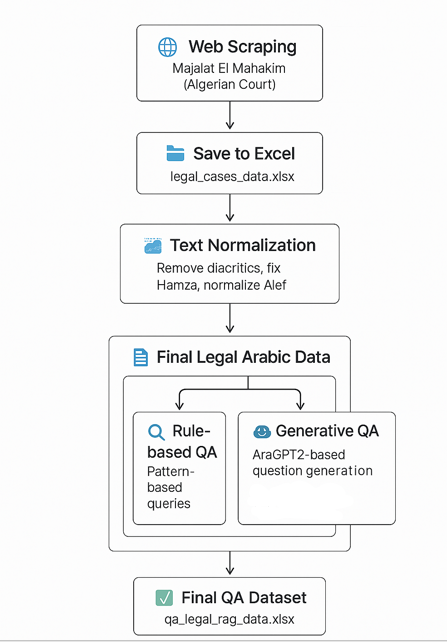
\includegraphics[width=0.5\linewidth]{Figures/dataC.png}
	\caption{The detailed pipeline used for the creation of both the legal case dataset and the  question-answer QA}
	\label{dataset_creation}
	
\end{figure}

\newpage
\section{Agent Architecture Overview}
To build an Arabic legal assistant capable of answering questions about legal cases, we adopted an agentic architecture based on  RAG. The Agent is composed of modular components that work together to understand user questions, retrieve relevant legal content, and generate informative responses. It is designed to handle complex legal texts and support both general legal queries and specific requests, such as extracting particular legal articles Figure~\ref{agentic_architecture} illustrates Agent Architecture Overview.
\begin{figure}[h]
	\centering
	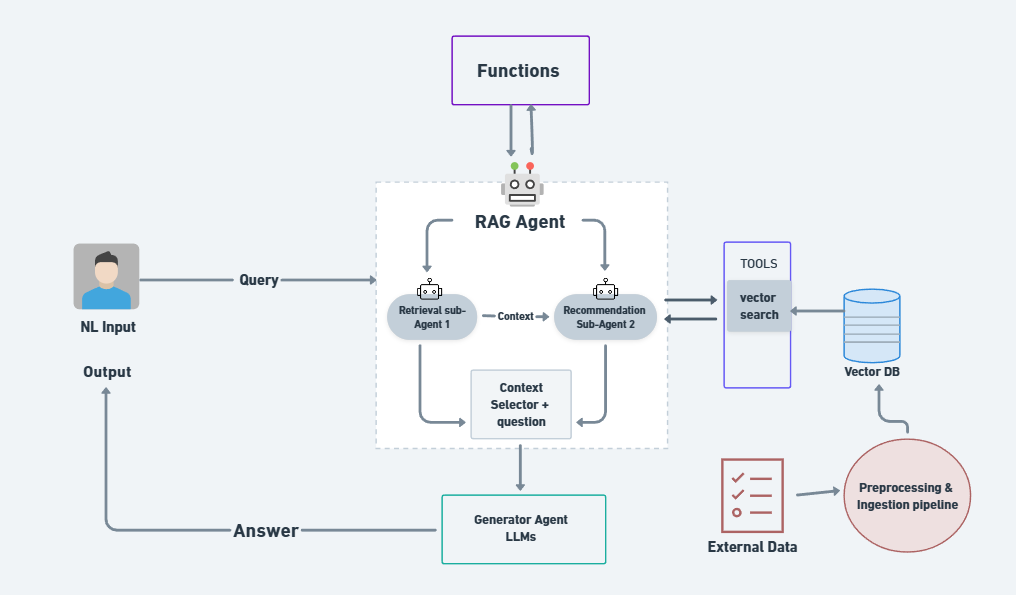
\includegraphics[width=0.9\linewidth]{Figures/agentarchi.png}
	\caption{Architecture of the Arabic RAG-Based Agent for Legal Data. The Agent takes Arabic natural-language questions as input and returns answers grounded in real legal case context. It integrates preprocessing, semantic retrieval, and generation agent. }
	
	\label{agentic_architecture}
	
\end{figure}

\subsection{Input/Output}

The agent \textbf{receives natural-language arabic questions as input}. These questions may range from general inquiries about a legal case to specific prompts requesting certain materials, such as legal articles. As output, the Agent\textbf{ returns either detailed answers grounded in real legal case context or a filtered subset of legal references} (e.g., materials/articles), depending on the nature of the user request.

\subsection{Preprocessing and Ingestion Phase}
Before retrieval and generation, legal documents go through a data ingestion pipeline. This includes cleaning and normalizing raw text, followed by semantic chunking to ensure each unit of information is appropriately sized. These chunks are then embedded and indexed into a vector database to enable efficient semantic retrieval during runtime. This phase ensures the quality, structure, and retrievability of legal content.

\subsection{Retriever Sub-Agent }
The retriever identifies the most relevant pieces of legal content based on the user’s query. It searches through the vectorized representation of the case database to return a ranked list of the most semantically similar chunks. This retrieval process ensures that the agent has access to high-quality and contextually relevant legal information.

\subsection{Recommendation Sub-Agent}
If the user's request targets specific legal materials (e.g., legal articles mentioned within a case), a recommendation sub-agent is triggered. This agent scans the previously retrieved content to identify and extract only the relevant sections that match patterns typically associated with legal article references. This sub-agent demonstrates intra-agent communication, as it relies on outputs from the main retriever while adding a specialized capability.
\subsection{Context Selector: Token-Aware Filtering}
From the retrieved candidates, the agent selects the most relevant chunks that fit within the system’s input constraints. This filtering ensures that the generator receives coherent, non-redundant, and contextually rich text to support accurate response generation.
\subsection{Functions and Tools}
In addition to the core RAG-based workflow, the architecture integrates a flexible function-calling and tool-use mechanism. This enables the agent to interact with external tools—such as file analyzers, legal databases. These tools are invoked dynamically based on the user query, and the outputs are fed back into the RAG Agent to support more grounded, context-aware answers.


\subsection{Generator: Answer Formulation Component}
Using the selected context, the generator produces a coherent and legally grounded answer in Arabic. The generation process is context-aware, allowing it to reflect the nuances of legal terminology and adapt the output style depending on the user’s request.

\subsection{Agent Design}
The core Agent functions as a domain-specific legal agent that uses Retrieval-Augmented Generation to assist users with legal case questions. It is capable of:

\begin{itemize}
	\item Understanding natural Arabic legal questions, including complex legal terminology.
	\item Retrieving relevant information from legal case texts using semantic search.
	\item Generating answers grounded in real legal content.
	\item Recommending specific legal materials when requested by the user.
\end{itemize}

Rather than relying on predefined responses, the agent dynamically retrieves and composes answers using the most relevant and up-to-date case context. It can be used by legal professionals, students, or institutions to enhance legal understanding and streamline research across a wide range of case types.
\section{Training the Agent}
To empower the Arabic RAG-Based Agent with accurate and context-aware responses, we trained both its retriever and generator components on a curated Arabic legal QA dataset. This training phase focused on optimizing the agent’s ability to understand user questions, retrieve the most relevant legal context, and generate coherent and grounded answers.
\begin{figure}[h]
	\centering
	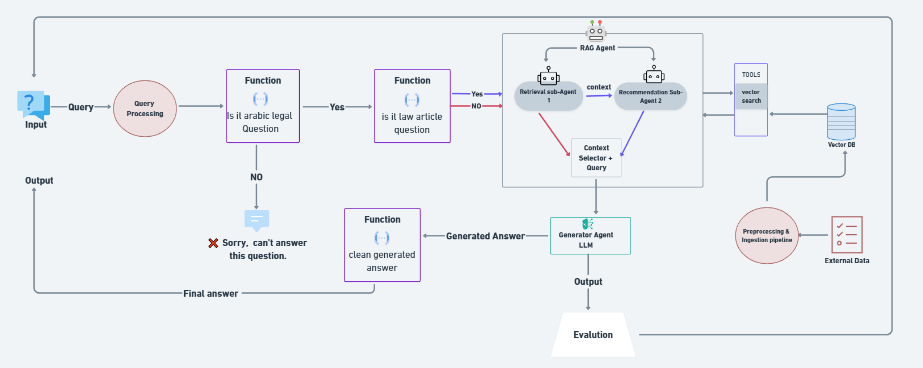
\includegraphics[width=0.8\linewidth]{Figures/trainingagent.png}
\caption{An overview of the training pipeline for the RAG agent }
	
	\label{agentic_trining}
	
\end{figure}


\subsection{Training the Retriever}
The retriever is responsible for identifying and retrieving the most relevant legal context for a given user query. This component can be trained or configured through several key phases that focus on data preprocessing, semantic embedding, and efficient indexing. Below, we outline a generalizable framework for training a dense retriever in Arabic legal RAG Agent.

\begin{itemize}
	\item \textbf{Text Normalization Pipeline:}
	A preprocessing stage is essential to clean and standardize Arabic legal texts. This may involve:
	\begin{itemize}
		\item Removing diacritics to minimize lexical variations.
		\item Normalizing common character variants (e.g., Alef, Taa Marbouta).
		\item Standardizing punctuation symbols and quotation marks.
		\item Eliminating excess whitespace and formatting inconsistencies.
	\end{itemize}
	
	\item \textbf{Document Chunking Strategy:}
	Legal documents are often lengthy and need to be divided into smaller, semantically coherent chunks. Common techniques include:
	\begin{itemize}
		\item Using recursive text splitters with a fixed token size (e.g., 300 or 500 tokens).
		\item Applying hierarchical splitting rules (paragraphs, then sentences, then phrases).
		\item Preserving key metadata like title, keywords, or article number.
		\item Leveraging tokenizer-based length calculation to ensure chunk boundaries match model requirements.
	\end{itemize}
	
	\item \textbf{Dense Retrieval Architecture:}
	Semantic search typically relies on encoding both documents and queries into dense vector representations using transformer-based models. Common considerations include:
	\begin{itemize}
		\item Choosing a pre-trained multilingual or Arabic-specific embedding model.
		\item Applying mean pooling or CLS token extraction to produce sentence-level embeddings.
		\item Normalizing embeddings (e.g., via L2 normalization) to improve similarity computation.
		\item Using batch processing for faster embedding generation on GPU or CPU.
	\end{itemize}
	
	\item \textbf{Indexing Framework:}
	To enable efficient similarity search, embedding vectors can be stored in a specialized vector database or indexing engine. Some popular practices include:
	\begin{itemize}
		\item Using FAISS or other vector stores to build inner-product or approximate nearest neighbor indices.
		\item Associating each embedding with its original text and metadata.
		\item Tracking chunk-document mappings for traceability during retrieval.
	\end{itemize}
	
	\item \textbf{Query Processing:}
	The user question must be preprocessed and embedded in the same way as documents. Key steps may involve:
	\begin{itemize}
		\item Prefixing or formatting the query to match model expectations.
		\item Applying the same normalization steps used during indexing.
		\item Calculating similarity scores (e.g., cosine similarity) between query and document vectors.
		\item Returning the top-k matching chunks with associated document IDs or metadata.
	\end{itemize}
	
	\item \textbf{Evaluation Dataset:}
	Evaluating retrieval quality typically involves a labeled dataset containing questions, gold answers, and corresponding contexts. This can be used to measure:
	\begin{itemize}
		\item Retrieval accuracy metrics such as :
		\begin{enumerate}
			\item  Recall@K measures the proportion of queries where the correct case appears in the top-K results,
			\item  MRR (Mean Reciprocal Rank) emphasizes the position of the first correct result through reciprocal weighting. 
			\item Hit@K provides a binary success indicator for each query. 
		\end{enumerate}
		\item Relevance of retrieved contexts with respect to the ground-truth legal passages.
		\item The impact of retrieval quality on downstream answer generation.
	\end{itemize}
\end{itemize}
\subsection{Training the Generator}
The generator is responsible for producing fluent, accurate Arabic responses based on the user’s question and the retrieved legal context. It can be built using a pre-trained Arabic causal language model such as AraGPT2 or decoder-based models like AraBERT (in encoder-decoder setups), which are fine-tuned on legal QA data.
\begin{itemize}

\item\textbf{Prompt Design}
A typical input format for generation includes a clearly structured prompt that merges the question and retrieved legal context:
\begin{verbatim}
	Question: [user query]
	Reference: [retrieved legal text]
	Answer:
\end{verbatim}
This structure helps the model understand the roles of each input component and generate contextually appropriate responses.

\item\textbf{Data Preparation}
Training data should be tokenized using a tokenizer compatible with the selected Arabic model. Common preprocessing steps include:
\begin{itemize}
	\item Automatic padding and truncation to fit model token limits (e.g.,512, 1024,2024 tokens)
	\item Insertion of special separator tokens between segments (e.g., between question and context)
	\item Filtering or adjusting samples that exceed the model’s maximum input length
\end{itemize}
\item\textbf{Model Fine-Tuning}
The selected Arabic language model—such as AraGPT2 for autoregressive generation or AraBERT in encoder-decoder setups—can be fine-tuned using supervised datasets consisting of paired questions, legal context, and answers. Fine-tuning enables the model to specialize in the legal domain and improve performance on complex queries.
\item\textbf{Training Process}
The fine-tuning process typically includes:
\begin{itemize}
	\item \textbf{Causal Language Modeling Objective:} Training the model to predict the next token in a sequence given previous tokens.
	\item \textbf{Teacher Forcing:} Providing the ground truth answer during training to improve convergence .
	\item \textbf{Decoding Strategies:} Techniques like beam search can be used during inference to generate more controlled responses, while repetition control (e.g., no-repeat n-grams) is applied to avoid redundant phrases.
\end{itemize}

\item\textbf{Quality Control}
To ensure reliable and relevant legal answers, post-processing steps may include:
\begin{itemize}
	\item Removing prompt artifacts or formatting leftovers from generation.
	\item Verifying the inclusion of key legal terms or references.
	\item Checking contextual alignment between the retrieved reference and the generated answer.
\end{itemize}

\item\textbf{Evaluation of the Generator}
To assess the quality of the generated answers from the we can conducted a quantitative evaluation using two commonly used metrics for natural language generation: \textbf{BLEU} and \textbf{BERTScore}.

\begin{itemize}
	\item \subsection*{BLEU (Bilingual Evaluation Understudy):}
	 BLEU measures the $n$-gram overlap between the generated text and the reference text. It is a precision-based metric often used in machine translation and QA evaluation\citep{papineni2002bleu}. In our experiment, we used the official implementation provided by the \texttt{sacrebleu} library to ensure reproducibility and standardization.
    \item \subsection*{BERTScore:}
	BERTScore computes similarity between the embeddings of the generated and reference sentences using a pretrained contextual language model \citep{zhang2019bertscore}(in our case, Arabic BERT). It provides precision, recall, and F1 scores. We report the average F1 score, which reflects semantic similarity rather than just surface overlap.
\end{itemize}
\end{itemize}
\section{Experimental Results}
The RAG Agent was rigorously validated through end-to-end testing and quantitative evaluation. Retrieval performance was measured confirming the retriever's ability to identify relevant legal cases and The generator was assessed through human evaluation and automated metrics for linguistic quality.
\subsection{Training Results}
During the training phase, the retriever and generator components were fine-tuned using a curated Arabic legal QA dataset. The retriever was trained to embed and index normalized document chunks using a dense semantic model, while the generator (based on AraGPT2) was trained on structured prompt-answer pairs. Both components were trained on colab T4 GPU due to limited GPU access, with careful preprocessing, batch management, and quality control applied throughout to ensure reliable convergence and domain-specific adaptation.


  	\subsubsection{Model Architecture}
The AraGPT2 architecture was selected for its ability to handle Arabic text generation while being computationally efficient. Below are the key specifications of the model:

\begin{table}[h]
	\centering
	
	\begin{tabular}{|l|l|}
		\hline
		\textbf{Component} & \textbf{Specification} \\ \hline
		Architecture & Decoder-only transformer \\ \hline
		Layers & 12 \\ \hline
		Hidden Size & 768 \\ \hline
		Attention Heads & 12 \\ \hline
		Parameters & 137M \\ \hline
		Vocabulary Size & 50,257 (Byte-level BPE) \\ \hline
		Max Position Embeddings & 1024 \\ \hline
	\end{tabular}
	\caption{ Core architectural specifications of the decoder-only transformer model used in this work}
\end{table}

	\subsubsection{Training Configuration}
The fine-tuning process employed carefully selected hyperparameters to balance training stability and model performance. The following table details the training setup:

\begin{table}[h]
	\centering
	
	\begin{tabular}{|l|l|}
		\hline
		\textbf{Parameter} & \textbf{Value} \\ \hline
		Batch Size & 2 (per device) \\ \hline
		Epochs & 20 \\ \hline
		Sequence Length & 1024 tokens \\ \hline
		Learning Rate & 5e-5 \\ \hline
		Weight Decay & 0.01 \\ \hline
		Gradient Accumulation & 1 \\ \hline
		Warmup Steps & 0 \\ \hline
		
	\end{tabular}
	\caption{Summary of key hyperparameters configured for model fine-tuning}
\end{table}
 

\subsubsection{Inference Settings}
At generation time, various hyperparameters influence output quality. Typical settings include:
\begin{itemize}
	\item \textbf{Maximum Output Length:} Capped to prevent overly long responses (e.g., 260 tokens).
	\item \textbf{Temperature:} Adjusts randomness in sampling (e.g., temperature = 1.0 for deterministic output).
	\item \textbf{Top-k/Top-p Sampling:} Can be enabled or disabled depending on the desired balance between creativity and consistency.
	\item \textbf{Penalties:} Repetition and length penalties help enforce concise and varied outputs.
\end{itemize}

 \subsubsection{Training Progress :}
The generator's training process was monitored using the training loss across epochs, as shown in the figure \ref{Training} below. 


\begin{figure}[h]
	\centering
	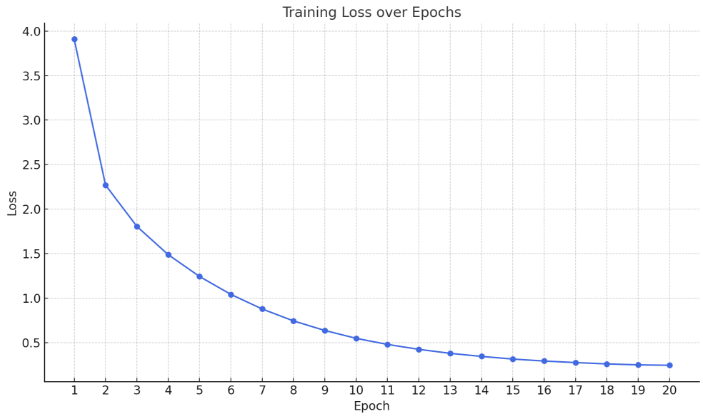
\includegraphics[width=0.7\linewidth]{Figures/finetunedresult.png}
	\caption{Training Loss over Epochs}
	\label{Training}
	
\end{figure}
The graph demonstrates a steady decline in loss, indicating that the model successfully learned from the data over time without signs of overfitting.

\newpage
\subsection{Evaluation Results}
The evaluation was conducted separately for both the retriever and generator components. For the retriever, we used a manually curated Arabic legal QA benchmark where each query was associated with gold-standard context passages. Retrieval performance was measured using standard top-k accuracy metrics, confirming that the Agent consistently retrieved the correct legal context within the top 3 results. For the generator, we evaluated the quality of generated answers using both human judgment and automatic metrics, focusing on fluency, legal accuracy, and relevance to the retrieved context. The results showed that the generator was capable of producing coherent Arabic answers that aligned well with the legal source material in most cases.
\subsection{Retriever Evaluation Results}
The retriever's effectiveness was quantitatively assessed using three standard information retrieval metrics computed across multiple top-K thresholds.
\begin{figure}[h]
	\centering
	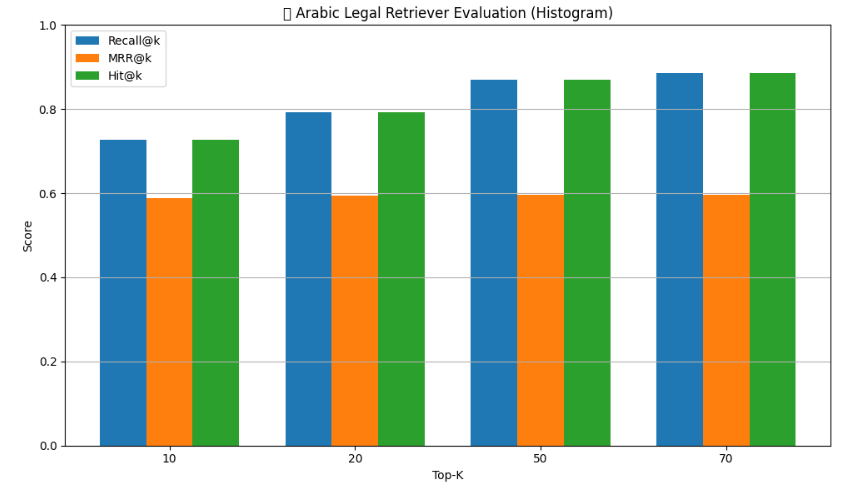
\includegraphics[width=0.8\textwidth]{Figures/evalutionhisto.png}
	\caption{Retrieval performance metrics across different top-K values. The histogram shows consistent improvement in Recall@K, MRR@K, and Hit@K as K increases.}
	\label{fig:retriever_performance}
\end{figure}

As shown in Figure~\ref{fig:retriever_performance}, performance scales with K, achieving 92\% Recall@70 and MRR@70 of  0.88, indicating both high coverage and quality of rankings. The evaluation protocol embedded each test query using the E5 model's  token representation, then searched the FAISS index for nearest neighbors. Case ID matching against the ground truth confirmed retrieval accuracy, with error analysis revealing most failures occurred for queries containing ambiguous legal terminology or incomplete case references.
\paragraph{Human Evaluation:}
The RAG agent was evaluated using a curated set of legal queries paired with ground-truth case IDs. For each query, the retriever generated top-k candidate passages (k=3), which were analyzed for correctness by comparing retrieved case IDs against the ground truth.\\

\begin{figure}[h]
	\centering
	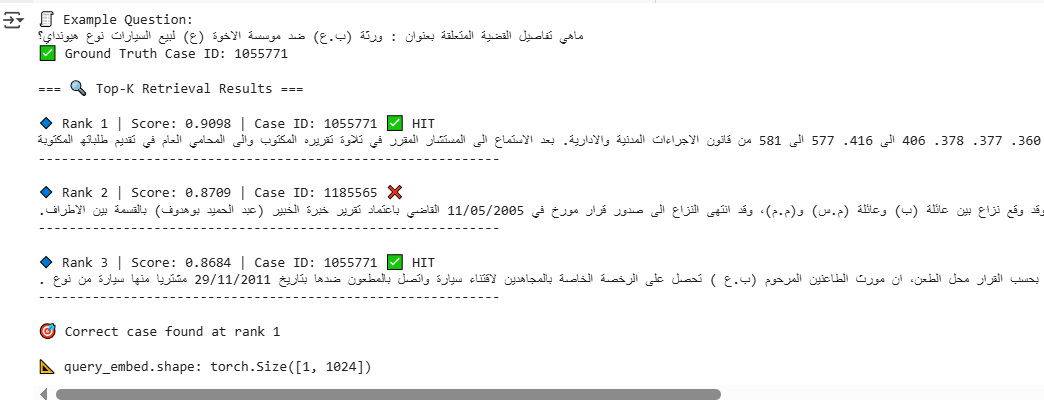
\includegraphics[width=0.8\linewidth]{Figures/testRs.png}
	\caption{Retrieval performance on a sample legal query showing the top-3 results with similarity scores. }
	\label{fig:retrieval_example}
\end{figure}
A representative  evaluation case (shown in Figure ~\ref{fig:retrieval_example} demonstrates successful retrieval, where the correct legal case (ID 1055771) was ranked first with a high similarity score (8.9098), significantly outperforming lower-ranked candidates (0.8789 and below).
\subsection{Geerator Evaluation Results }
We ran our \texttt{rag\_pipeline} function on each question in the legal QA dataset, collected the generated answers, and compared them to the ground truth answers using both metrics.

\paragraph{Results:}
\begin{itemize}
	\item \textbf{BLEU Score (official):} 27.33
	\item \textbf{BERTScore F1 Average:} 0.7903
\end{itemize}

These results suggest that the generator produces contextually accurate and semantically relevant answers, with moderate lexical overlap and high embedding-level similarity.
\paragraph{Human Evaluation:}

To complement automatic evaluation metrics such as BLEU and BERTScore, we conducted a human evaluation through the deployed Arabic legal assistant interface.

\begin{figure}[H]
	\centering
	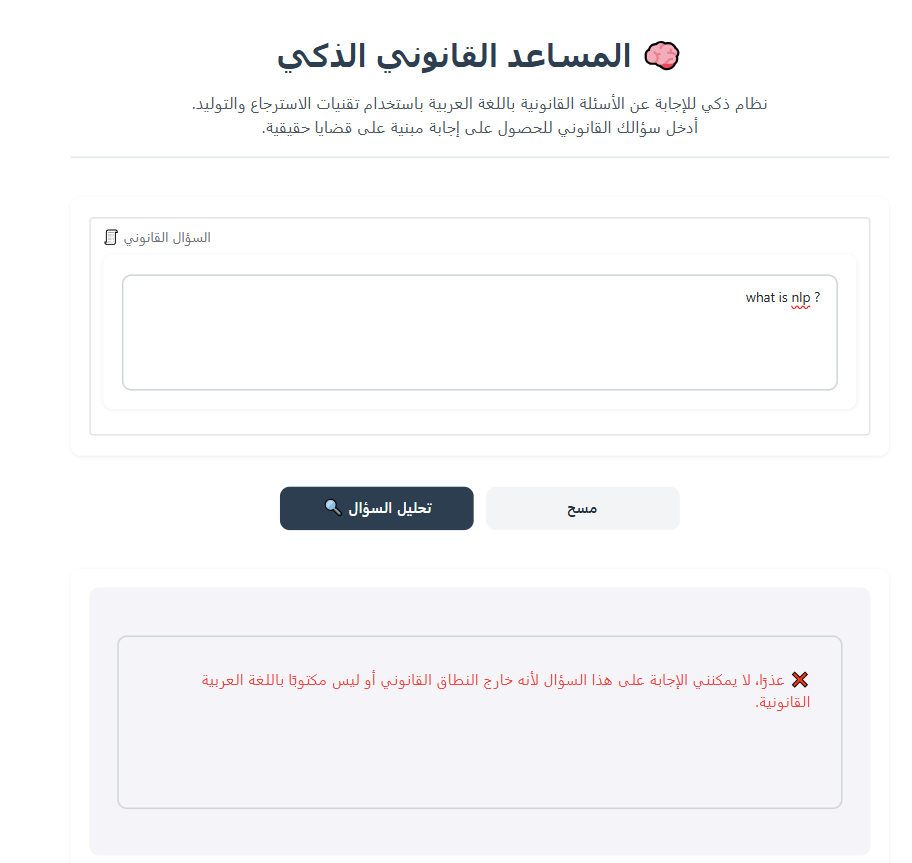
\includegraphics[width=0.7\textwidth]{Figures/evalG.png}
	\caption{An example from the Arabic legal assistant interface showing rejection of an irrelevant question ("What is NLP?") because it is not written in formal Arabic. This reflects the Agent ability to filter non-domain input during inference.}
	\label{fig_human_eval_example}
\end{figure}

As illustrated in Figure~\ref{fig_human_eval_example}, the Agent is able to identify and reject inputs that are unrelated to the legal domain. This behavior ensures that the assistant remains focused on legal queries, aligning with the intended use-case and improving reliability in real-world usage.

\section{Agent Results}
This section presents the user interface of the intelligent legal agent after integrating all RAG components. The interface allows users to input Arabic legal questions and receive automatically generated answers based on retrieved real legal cases. A screenshot of the final application is shown below, demonstrating the usability and functionality of the Agent in action. Users can input their questions, process them via a backend RAG pipeline, and view the results in a styled and intuitive format.
\begin{itemize}
	\item \textbf{Intelligent Legal Agent Interface :}\\
   The interface allows users to input legal questions in Arabic and receive accurate answers based on real legal case data.\\
   Figure\ref{inter} highlights the main components of the interface, including the input field for questions, control buttons, and the answer display box.

\begin{figure}[h]
	\centering
	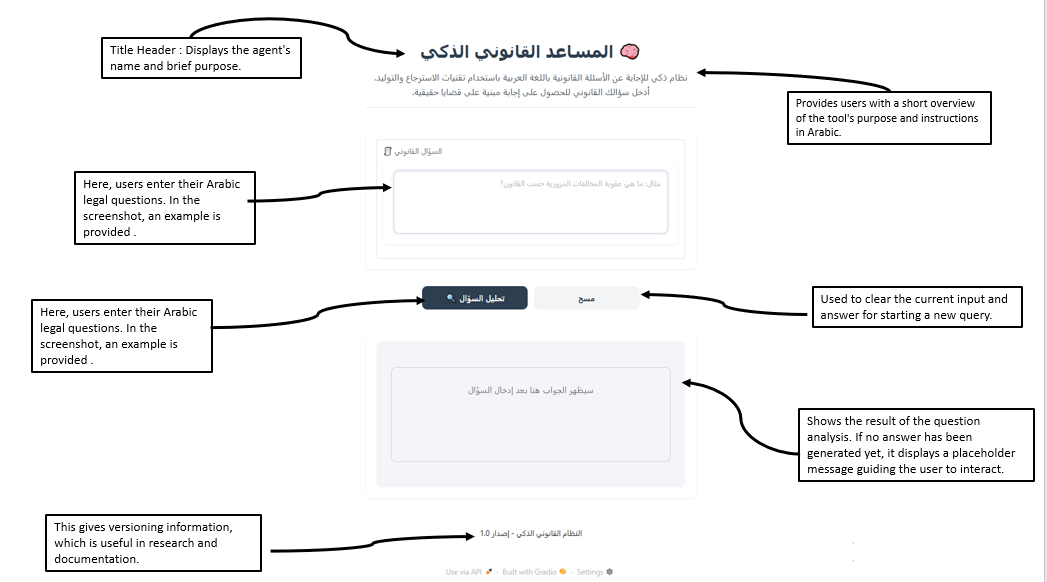
\includegraphics[width=0.9\textwidth]{Figures/interagent.png}
	\caption{ Interactive interface of the Intelligent Legal Assistant Agent.}
	\label{inter}
\end{figure}
\item \textbf{Detailed Case Answering via RAG Agent}
Figure\ref{legal_rag_interface} shows the user interface of the Arabic Legal RAG  Agent. In this example, the user inputs a general query asking for the details of a case based on its title.
\begin{figure}[H]
	\centering
	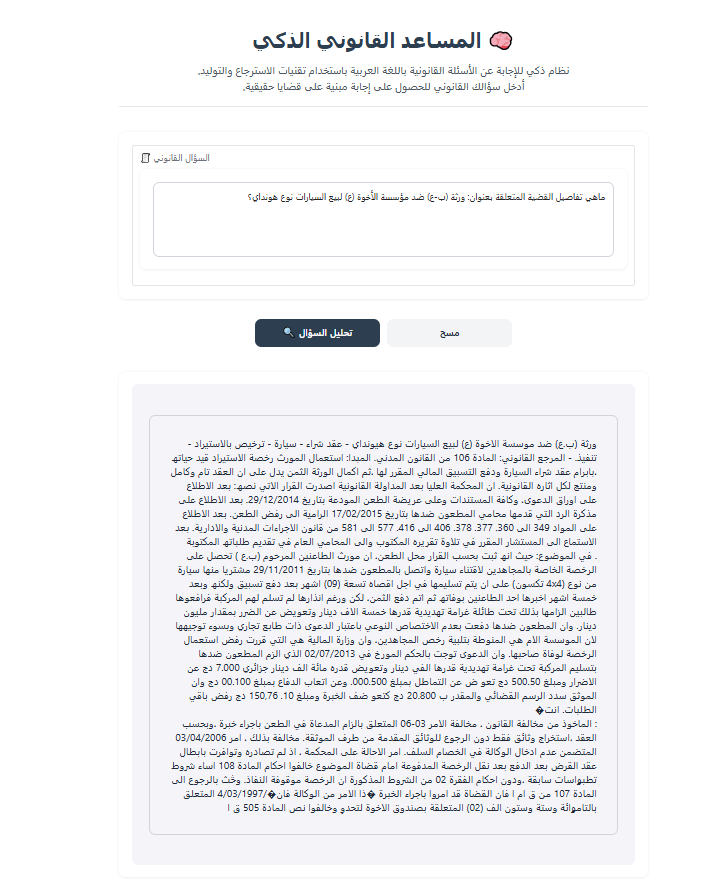
\includegraphics[width=0.6\textwidth]{Figures/answer.png}
	\caption{Interface of the Arabic Legal RAG Assistant showing a successful answer to a general legal query using the case title. The Agent retrieves relevant case data and generates a comprehensive legal response .}
	\label{legal_rag_interface}
\end{figure}

The RAG Agent retrieves the most relevant case chunks using semantic search  and generates a detailed answer using the AraGPT2 model. The response includes important legal information such as contract type, legal articles, procedural details, and court decisions. The generated text is complete, accurate, and contextually grounded, demonstrating the Agent’s ability to handle vague or broad legal questions and return precise, useful answers.

\end{itemize}

%%=============================================%%
\newpage
\section{Conclusion}
In this chapter, we presented the complete development pipeline of an Arabic Retrieval-Augmented Generation (RAG) based agent tailored for legal question answering. The Agent was constructed through a sequence of carefully designed components, starting from data collection and preprocessing of Arabic legal documents and QA pairs, followed by the construction of a dense retriever using FAISS and the multilingual E5 encoder. We then integrated a generator—fine-tuned AraGPT2—to synthesize accurate answers grounded in retrieved legal context.

We evaluated the retriever independently using retrieval metrics such as Recall@k and MRR,  Subsequently, the generator was evaluated using both automatic metrics—BLEU and BERTScore—and human evaluation through a controlled interface.

Overall, the developed RAG-based Agent provides a solid foundation for intelligent legal assistance in Arabic. It not only bridges the gap between dense retrieval and controlled generation but also offers a scalable framework for future enhancements such as domain expansion, re-ranking modules, or multilingual capabilities.






		\chapter*{Conclusion}
\pagestyle{fancy}\lhead{\textbf \footnotesize\it{Conclusion}}
\pagestyle{fancy}\chead{} \pagestyle{fancy}\rhead{}
\pagestyle{fancy}\cfoot{} \pagestyle{fancy}\rfoot{\thepage}
%\addcontentsline{toc}{chapter}{General conclusion}
%%%%%%%%%%%%%%%%%%%%%%%%%%%%%%%%%%%% 
This thesis has investigated the intersection of natural language processing technologies and the legal domain, with a particular focus on the capabilities and limitations of large-scale language models in processing complex Arabic legal texts. We began by presenting a foundational overview of Large Language Models (LLMs), exploring their potential for legal text understanding and generation, while also highlighting the specific challenges they face in dynamic, high-stakes environments. Following this, we introduced the concept of Agentic AI, outlining its general characteristics and its emerging role in enabling autonomous, goal-driven reasoning.

To address the limitations of static language models, we turned to RAG architectures, which enhance language models by integrating external document retrieval systems. This hybrid approach offers a more grounded and context-aware solution, crucial for legal question answering and reasoning tasks

Chapter 3 addressed one of the core limitations of traditional RAG systems: the use of fixed top-k document selection. We proposed a dynamic candidate selection mechanism that adjusts the retrieval scope based on the complexity of the user query, thereby improving retrieval precision and reducing noise in the generation process.

In Chapter 4, these concepts were brought together in a fully implemented Arabic RAG pipeline. This included preprocessing, semantic embedding, FAISS-based indexing, and generation using a fine-tuned model. The resulting conversational agent enables natural language querying of Algerian legal content and delivers grounded, contextually relevant answers. Additionally, the thesis introduced a curated dataset of Algerian legal cases in Arabic, addressing a major gap in Arabic legal NLP resources.

Overall, this work offers both theoretical contributions and practical tools for advancing legal AI in under-resourced settings. By combining dynamic retrieval, generation, and agentic reasoning, the thesis lays the groundwork for the next generation of intelligent legal assistants in the Arab world.

%\newpage







	%%%%%%%%%%%%%%%%%%%%% For bibliography %%%%%%%%%%%%%%%%%%
	\newpage
  % Before babel if using author-year
 \bibliographystyle{plainnat}
	\bibliography{Biblio}
	\pagestyle{fancy}\lhead{\textbf \footnotesize\it{Bibliography}}
	\pagenumbering{gobble} % To suppress numbering 
	%\addcontentsline{toc}{chapter}{Bibliography}
	%%%%%%%%%%%%%%%%%%%%% For appendices %%%%%%%%%%%%%%%%%%%
	%\appendix
		%
\pagestyle{fancy}\lhead{\textbf \footnotesize\it{Selected Large Language Models}}
\pagestyle{fancy}\rhead{\textbf \footnotesize\it{}}
\pagenumbering{gobble}
%%%%%%%%%%%%%%%%%%%%%%%%%%%%%%%%%%%%%%%%%%%%%

\newpage% Appendix A
	% ====== Appendix Section ======

\appendix
\chapter*{Appendix}  % Unnumbered chapter
\pagestyle{fancy}
\lhead{\textbf{\footnotesize\itshape Appendix}}  % Left header
\rhead{}  % Right header empty
\pagenumbering{gobble}  % Turn off page numbering

% Include the PDF ON THE SAME PAGE
\vspace*{-3em}  % Pulls the PDF up closer to the title (adjust as needed)
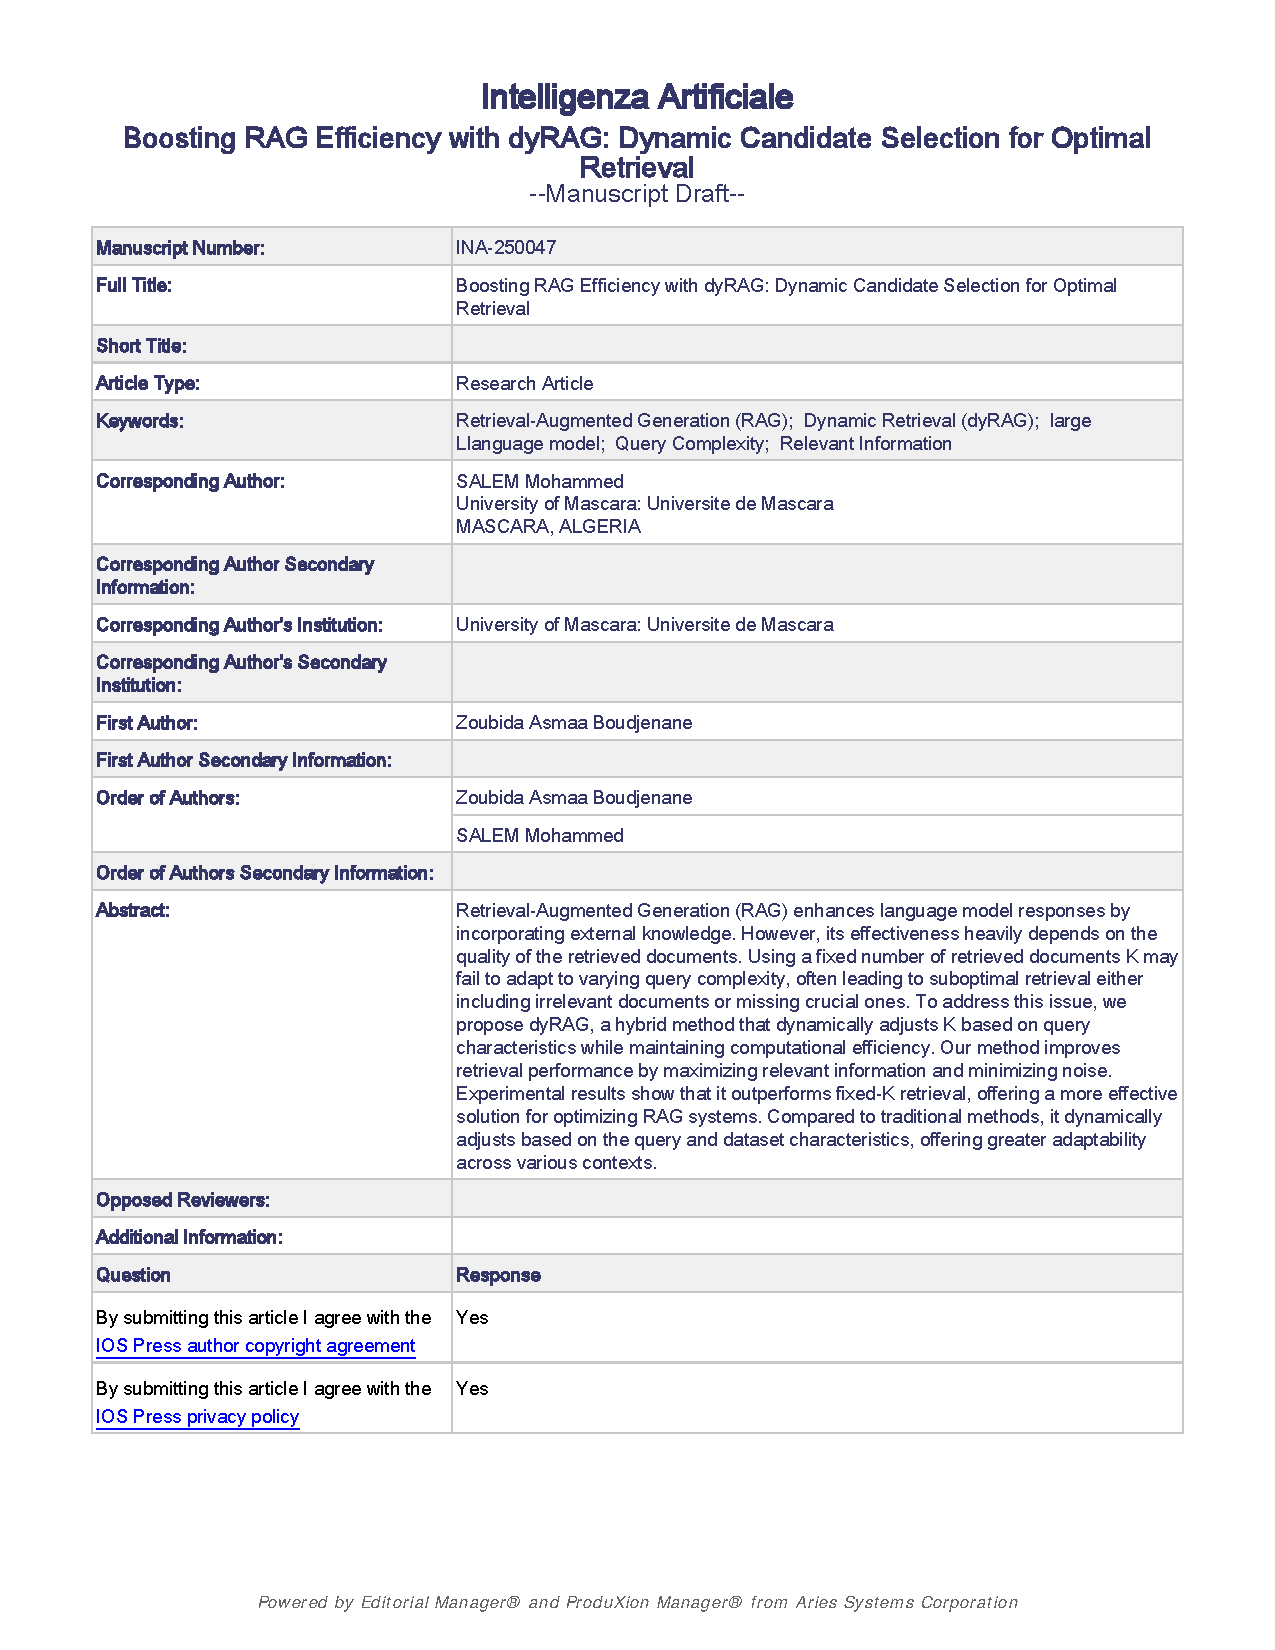
\includepdf[
pages=-,
scale=0.8,
pagecommand={},  % Remove automatic page styling
offset=0 -1cm,  % Fine-tune vertical position
  % Optional: Add border for debugging
]{INA-250047.pdf}% Appendix B
	%\addcontentsline{toc}{chapter}{Appendices}
\end{document}